% ============================================================
% The Building Blocks of LLMs: A Mathematical History
% CONDENSED 30-SLIDE VERSION (standalone)
% From Archimedes to Attention: 2,000+ Years of Mathematics Inside Your AI
% Target Audience: High School Seniors (Mathematics)
% Duration: ~40-45 minutes
% ============================================================
\documentclass[aspectratio=169,12pt]{beamer}

% ---- Theme & Colors ----
\usetheme{Madrid}
\usecolortheme{whale}

% Custom color palette (shared with main lecture)
\definecolor{babylonBrown}{RGB}{139,90,43}
\definecolor{greekBlue}{RGB}{0,71,171}
\definecolor{indianSaffron}{RGB}{204,119,34}
\definecolor{chineseRed}{RGB}{170,56,30}
\definecolor{islamicGreen}{RGB}{0,128,55}
\definecolor{medievalPurple}{RGB}{102,51,153}
\definecolor{renaissanceGold}{RGB}{184,134,11}
\definecolor{enlightenmentTeal}{RGB}{0,128,128}
\definecolor{modernSteel}{RGB}{70,130,180}
\definecolor{digitalBlue}{RGB}{30,80,162}
\definecolor{aiViolet}{RGB}{106,13,173}
\definecolor{accentOrange}{RGB}{230,126,34}
\definecolor{darkBg}{RGB}{30,30,30}

% LLM-specific section colors
\definecolor{linalgTeal}{RGB}{0,150,136}
\definecolor{calculusRed}{RGB}{211,47,47}
\definecolor{probBlue}{RGB}{25,118,210}
\definecolor{infoAmber}{RGB}{255,160,0}
\definecolor{logicGray}{RGB}{97,97,97}
\definecolor{approxGreen}{RGB}{56,142,60}
\definecolor{neuronPink}{RGB}{194,24,91}
\definecolor{seqIndigo}{RGB}{63,81,181}

% Set main beamer colors - aiViolet as primary
\setbeamercolor{palette primary}{bg=aiViolet,fg=white}
\setbeamercolor{palette secondary}{bg=aiViolet!80,fg=white}
\setbeamercolor{palette tertiary}{bg=aiViolet!60,fg=white}
\setbeamercolor{frametitle}{bg=aiViolet,fg=white}
\setbeamercolor{title}{bg=aiViolet,fg=white}
\setbeamercolor{section in toc}{fg=aiViolet}
\setbeamercolor{block title}{bg=aiViolet,fg=white}
\setbeamercolor{block body}{bg=aiViolet!5}
\setbeamercolor{item}{fg=aiViolet}

% ---- Fonts ----
\usefonttheme{professionalfonts}
\setbeamerfont{title}{size=\Large,series=\bfseries}
\setbeamerfont{frametitle}{size=\large,series=\bfseries}
\setbeamerfont{framesubtitle}{size=\normalsize,series=\mdseries}

% ---- Packages ----
\usepackage[utf8]{inputenc}
\usepackage[T1]{fontenc}
\usepackage{amsmath,amssymb,amsfonts}
\usepackage{graphicx}
\usepackage{tikz}
\usetikzlibrary{shapes,arrows.meta,positioning,calc,decorations.pathmorphing,backgrounds,fit}
\usepackage{booktabs}
\usepackage{multicol}
\usepackage{hyperref}
\usepackage{fontawesome5}
\usepackage{xcolor}
\usepackage{pgfplots}
\pgfplotsset{compat=1.18}
\usepackage{tcolorbox}
\tcbuselibrary{skins,breakable}

% ---- Custom Commands ----

% Person info box
\newtcolorbox{personbox}[2][]{%
  colback=#2!5,
  colframe=#2,
  fonttitle=\bfseries,
  title=#1,
  rounded corners,
  boxrule=1pt,
  left=4pt,right=4pt,top=4pt,bottom=4pt
}

% Key insight callout
\newtcolorbox{insightbox}{%
  colback=accentOrange!10,
  colframe=accentOrange,
  fonttitle=\bfseries,
  title={\faLightbulb\ Key Insight},
  rounded corners,
  boxrule=1pt,
  left=4pt,right=4pt,top=4pt,bottom=4pt
}

% Connection to LLM callout
\newtcolorbox{llmconnection}{%
  colback=aiViolet!8,
  colframe=aiViolet,
  fonttitle=\bfseries,
  title={\faRobot\ Inside the LLM},
  rounded corners,
  boxrule=1pt,
  left=4pt,right=4pt,top=4pt,bottom=4pt
}

% Convergence progress bar
\newcommand{\convergencebar}[1]{%
  \begin{tcolorbox}[colframe=aiViolet!60, colback=white, boxrule=0.5pt,
    width=\textwidth, left=2pt, right=2pt, top=2pt, bottom=2pt]
  \centering\small\textbf{Building Blocks Found: #1 / 10}\\[4pt]
  \ifnum#1>0 \textcolor{linalgTeal}{\rule{8pt}{8pt}}\else\textcolor{gray!30}{\rule{8pt}{8pt}}\fi\hspace{2pt}%
  \ifnum#1>1 \textcolor{calculusRed}{\rule{8pt}{8pt}}\else\textcolor{gray!30}{\rule{8pt}{8pt}}\fi\hspace{2pt}%
  \ifnum#1>2 \textcolor{probBlue}{\rule{8pt}{8pt}}\else\textcolor{gray!30}{\rule{8pt}{8pt}}\fi\hspace{2pt}%
  \ifnum#1>3 \textcolor{infoAmber}{\rule{8pt}{8pt}}\else\textcolor{gray!30}{\rule{8pt}{8pt}}\fi\hspace{2pt}%
  \ifnum#1>4 \textcolor{logicGray}{\rule{8pt}{8pt}}\else\textcolor{gray!30}{\rule{8pt}{8pt}}\fi\hspace{2pt}%
  \ifnum#1>5 \textcolor{approxGreen}{\rule{8pt}{8pt}}\else\textcolor{gray!30}{\rule{8pt}{8pt}}\fi\hspace{2pt}%
  \ifnum#1>6 \textcolor{neuronPink}{\rule{8pt}{8pt}}\else\textcolor{gray!30}{\rule{8pt}{8pt}}\fi\hspace{2pt}%
  \ifnum#1>7 \textcolor{seqIndigo}{\rule{8pt}{8pt}}\else\textcolor{gray!30}{\rule{8pt}{8pt}}\fi\hspace{2pt}%
  \ifnum#1>8 \textcolor{aiViolet}{\rule{8pt}{8pt}}\else\textcolor{gray!30}{\rule{8pt}{8pt}}\fi\hspace{2pt}%
  \ifnum#1>9 \textcolor{accentOrange}{\rule{8pt}{8pt}}\else\textcolor{gray!30}{\rule{8pt}{8pt}}\fi%
  \end{tcolorbox}
}

% Verify tag (for speaker notes)
\newcommand{\verifytag}[1]{\textcolor{red!70}{\textbf{[VERIFY:} \textit{#1}\textbf{]}}}

% Slide counter in footline
\setbeamertemplate{footline}{%
  \leavevmode%
  \hbox{%
    \begin{beamercolorbox}[wd=.333333\paperwidth,ht=2.25ex,dp=1ex,center]{author in head/foot}%
      \usebeamerfont{author in head/foot}\insertshortauthor
    \end{beamercolorbox}%
    \begin{beamercolorbox}[wd=.333333\paperwidth,ht=2.25ex,dp=1ex,center]{title in head/foot}%
      \usebeamerfont{title in head/foot}\insertshorttitle
    \end{beamercolorbox}%
    \begin{beamercolorbox}[wd=.333333\paperwidth,ht=2.25ex,dp=1ex,right]{date in head/foot}%
      \usebeamerfont{date in head/foot}\insertframenumber{} / \inserttotalframenumber\hspace*{2ex}
    \end{beamercolorbox}}%
  \vskip0pt%
}

% Remove navigation symbols
\setbeamertemplate{navigation symbols}{}

% Tighten vertical spacing below frame titles
\addtobeamertemplate{frametitle}{}{\vspace{-0.3em}}

% ---- Document Info ----
\title[Building Blocks of LLMs]{The Building Blocks of LLMs\\[0.3em]{\large A Mathematical History}}
\subtitle{2,000+ Years of Mathematics Inside Your AI}
\author{Prof.\ J.\ Osterrieder}
\date{2026}
\institute{}

% ============================================================
\begin{document}

% ============================================================
% SLIDE 1: Title
% ============================================================
\begin{frame}[plain]
  \begin{tikzpicture}[remember picture, overlay]
    \fill[aiViolet] (current page.south west) rectangle (current page.north east);
  \end{tikzpicture}

  \vspace{1cm}
  \begin{center}
    {\Huge\bfseries\textcolor{white}{The Building Blocks of LLMs}}\\[0.6em]
    {\Large\textcolor{white!90}{A Mathematical History}}\\[1.5em]
    {\large\textcolor{white!80}{From Archimedes to Attention:}}\\[0.3em]
    {\large\textcolor{white!80}{2,000+ Years of Mathematics Inside Your AI}}\\[2em]
    {\normalsize\textcolor{white!70}{Prof.\ J.\ Osterrieder \hspace{2em} 2026}}
  \end{center}

  \note{
    NOW: You talk to AI every day. THEN: We are about to travel back through
    2,000 years of mathematics to find out where every piece came from.

    ``Welcome. This is not about hype or `intelligence.' This is about tracing
    every mathematical component of the AI you use daily back to the person
    who invented it --- often centuries before AI existed.''
  }
\end{frame}


% ============================================================
% SLIDE 2: What's Inside Your AI?
% ============================================================
\begin{frame}{What's Inside Your AI?}

  \begin{columns}[T]
    \begin{column}{0.46\textwidth}
      \vspace{0.1em}
      {\small When you type a question to ChatGPT or Claude\ldots}

      \vspace{0.1em}
      {\small The machine that answers is built \alert{entirely from mathematics}.}

      \vspace{0.1em}
      {\small
      \begin{itemize}\setlength\itemsep{0pt}
        \item Not magic
        \item Not ``intelligence''
        \item \textbf{Specific math}, invented by \textbf{specific people},
              at \textbf{specific times}
      \end{itemize}}

      \vspace{0.1em}
      \begin{tcolorbox}[colback=accentOrange!10, colframe=accentOrange,
        fonttitle=\bfseries, title={\faLightbulb\ Key Insight},
        rounded corners, boxrule=1pt, left=3pt, right=3pt, top=2pt, bottom=2pt]
        \small You already know some of this math.
        You just don't know it's inside your AI yet.
      \end{tcolorbox}
    \end{column}

    \begin{column}{0.50\textwidth}
      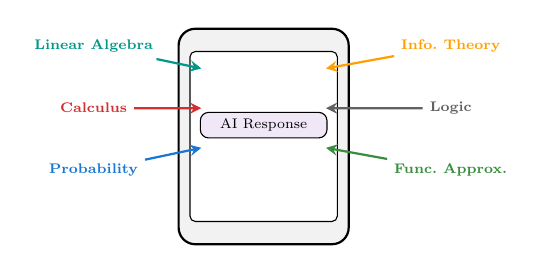
\begin{tikzpicture}[scale=0.72, every node/.style={transform shape},
        every node/.append style={font=\scriptsize\bfseries},
        arr/.style={->,>=stealth,thick}
      ]
        % Smartphone outline
        \draw[rounded corners=6pt, thick, fill=gray!10]
          (0,0) rectangle (3,3.8);
        \draw[rounded corners=2pt, fill=white]
          (0.2,0.4) rectangle (2.8,3.4);
        % Chat bubble inside
        \node[draw, rounded corners=3pt, fill=aiViolet!10,
              text width=2cm, align=center, font=\scriptsize]
          (chat) at (1.5,2.1) {AI Response};
        % Six labeled arrows from outside pointing in
        \node[text=linalgTeal] (la) at (-1.5,3.5) {Linear Algebra};
        \draw[arr, linalgTeal] (la) -- (0.4,3.1);
        \node[text=calculusRed] (ca) at (-1.5,2.4) {Calculus};
        \draw[arr, calculusRed] (ca) -- (0.4,2.4);
        \node[text=probBlue] (pr) at (-1.5,1.3) {Probability};
        \draw[arr, probBlue] (pr) -- (0.4,1.7);
        \node[text=infoAmber] (it) at (4.8,3.5) {Info.\ Theory};
        \draw[arr, infoAmber] (it) -- (2.6,3.1);
        \node[text=logicGray] (lo) at (4.8,2.4) {Logic};
        \draw[arr, logicGray] (lo) -- (2.6,2.4);
        \node[text=approxGreen] (fa) at (4.8,1.3) {Func.\ Approx.};
        \draw[arr, approxGreen] (fa) -- (2.6,1.7);
      \end{tikzpicture}
    \end{column}
  \end{columns}

  \note{
    NOW: Your phone, right now, runs a machine built from 10 branches of
    mathematics. THEN: Each branch was invented by a specific person, at a
    specific time, for a reason that had nothing to do with AI.

    ``You already know some of this math. You just don't know it's inside
    your AI yet. Today we're going to fix that.''
  }
\end{frame}


% ============================================================
% SLIDE 3: The Roadmap
% ============================================================
\begin{frame}{The Roadmap --- Ten Streams, One Machine}

  \convergencebar{0}

  \vspace{0.3em}
  \begin{center}
  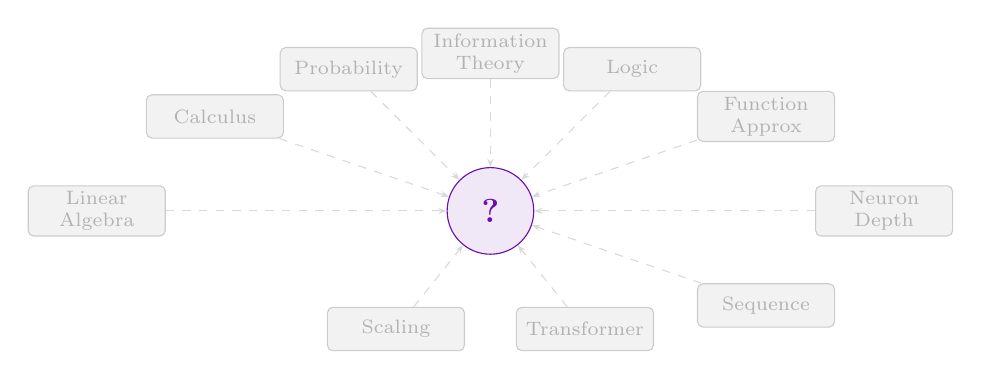
\begin{tikzpicture}[
    every node/.style={font=\scriptsize, align=center, minimum height=0.55cm,
      rounded corners=2pt, inner sep=2pt},
    dim/.style={draw=gray!40, fill=gray!10, text=gray!60}
  ]
    \node[dim, text width=1.6cm] (n1) at (-5,0) {Linear\\Algebra};
    \node[dim, text width=1.6cm] (n2) at (-3.5,1.2) {Calculus};
    \node[dim, text width=1.6cm] (n3) at (-1.8,1.8) {Probability};
    \node[dim, text width=1.6cm] (n4) at (0,2) {Information\\Theory};
    \node[dim, text width=1.6cm] (n5) at (1.8,1.8) {Logic};
    \node[dim, text width=1.6cm] (n6) at (3.5,1.2) {Function\\Approx};
    \node[dim, text width=1.6cm] (n7) at (5,0) {Neuron\\Depth};
    \node[dim, text width=1.6cm] (n8) at (3.5,-1.2) {Sequence};
    \node[dim, text width=1.6cm] (n9) at (1.2,-1.5) {Transformer};
    \node[dim, text width=1.6cm] (n10) at (-1.2,-1.5) {Scaling};
    % Center
    \node[draw=aiViolet, fill=aiViolet!10, circle, minimum size=1.1cm,
      font=\large\bfseries, text=aiViolet] (ctr) at (0,0) {?};
    % Dashed arrows
    \draw[-{Stealth[length=3pt]}, gray!30, dashed] (n1) -- (ctr);
    \draw[-{Stealth[length=3pt]}, gray!30, dashed] (n2) -- (ctr);
    \draw[-{Stealth[length=3pt]}, gray!30, dashed] (n3) -- (ctr);
    \draw[-{Stealth[length=3pt]}, gray!30, dashed] (n4) -- (ctr);
    \draw[-{Stealth[length=3pt]}, gray!30, dashed] (n5) -- (ctr);
    \draw[-{Stealth[length=3pt]}, gray!30, dashed] (n6) -- (ctr);
    \draw[-{Stealth[length=3pt]}, gray!30, dashed] (n7) -- (ctr);
    \draw[-{Stealth[length=3pt]}, gray!30, dashed] (n8) -- (ctr);
    \draw[-{Stealth[length=3pt]}, gray!30, dashed] (n9) -- (ctr);
    \draw[-{Stealth[length=3pt]}, gray!30, dashed] (n10) -- (ctr);
  \end{tikzpicture}
  \end{center}

  \vspace{-0.3em}
  {\small\centering Ten branches of mathematics. 2,000+ years. All converging in one architecture.\par}

  \note{
    NOW: This diagram shows ten streams flowing into your AI.
    THEN: We start our first jump --- to a German schoolteacher in 1844
    whom nobody read.

    ``We're going to light up these nodes one by one. Each one is a piece
    of math that somebody invented, often for a completely different purpose,
    that ended up inside the machines you use every day.''
  }
\end{frame}


% ============================================================
% SLIDE 4: Linear Algebra -- Vectors, Matrices, and Words
% ============================================================
\section{Linear Algebra}
\begin{frame}{Vectors, Matrices, and Words}

  \begin{columns}[T]
    \begin{column}{0.55\textwidth}
      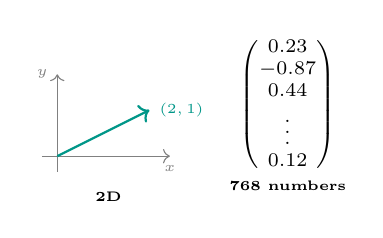
\begin{tikzpicture}[scale=0.65]
        % 2D vector
        \draw[->,gray,thin] (-0.3,0)--(2.2,0) node[below,font=\tiny]{$x$};
        \draw[->,gray,thin] (0,-0.3)--(0,1.6) node[left,font=\tiny]{$y$};
        \draw[->,thick,linalgTeal] (0,0)--(1.8,0.9)
          node[right,font=\tiny]{$(2,1)$};
        \node[below,font=\tiny\bfseries] at (1,-.5) {2D};
        % 768-dim column vector
        \begin{scope}[xshift=4.5cm, yshift=0.2cm]
          \node[font=\scriptsize,align=center] at (0,0.8)
            {$\begin{pmatrix}0.23\\-0.87\\0.44\\\vdots\\0.12\end{pmatrix}$};
          \node[below,font=\tiny\bfseries] at (0,-0.5) {768 numbers};
        \end{scope}
      \end{tikzpicture}

      \vspace{0.3em}
      {\small A \textbf{vector} = list of numbers. In an LLM, each word becomes
       a vector of 768+ numbers.}

      \vspace{0.3em}
      {\small A \textbf{matrix} = grid of numbers. Each neural network layer
       = matrix multiplication.}

      \vspace{0.2em}
      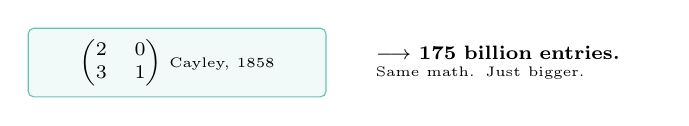
\begin{tikzpicture}
        \node[draw=linalgTeal!60, fill=linalgTeal!5, rounded corners=2pt,
              inner sep=4pt, text width=3.5cm, align=center, font=\scriptsize]
          {$\begin{pmatrix}2 & 0\\3 & 1\end{pmatrix}$
           {\tiny Cayley, 1858}};
        \node[font=\scriptsize, right, text width=3.5cm, align=left] at (2.4,0)
          {$\longrightarrow$ \textbf{175 billion entries.}\\[-2pt]
           {\tiny Same math. Just bigger.}};
      \end{tikzpicture}
    \end{column}

    \begin{column}{0.42\textwidth}
      \begin{tcolorbox}[colback=linalgTeal!5, colframe=linalgTeal,
        fonttitle=\bfseries\small, title={The Inventors},
        rounded corners, boxrule=0.8pt, left=3pt, right=3pt, top=2pt, bottom=2pt]
        \scriptsize
        \textbf{Grassmann} (1844)\\
        Schoolteacher. First general vector spaces.
        Nobody read his book.\\[2pt]
        \textbf{Cayley} (1858)\\
        Lawyer-turned-mathematician. Matrices as algebra.\\[2pt]
        \textbf{Sylvester} (1850)\\
        Coined ``matrix'' from Latin for ``womb.''\\[2pt]
        \textbf{Gauss} (1809)\\
        Gaussian elimination --- solving linear systems.
      \end{tcolorbox}

      \vspace{0.15em}
      \begin{llmconnection}
        \scriptsize
        96 layers $\times$ matrix multiply = how ChatGPT generates every word.
      \end{llmconnection}
    \end{column}
  \end{columns}

  \note{
    NOW: Every message you send to ChatGPT passes through 96 matrix multiplications.
    THEN: 1844, Stettin, Prussia --- Grassmann publishes a book so abstract nobody
    reads it. 1850 --- Sylvester coins ``matrix.'' Their inventions ARE the engine
    of modern AI.

    ``Grassmann was a schoolteacher nobody read. Sylvester named it `matrix' from
    Latin for `womb' --- he thought of it as something that gives birth to numbers.
    He had no idea it would give birth to AI.''
  }
\end{frame}


% ============================================================
% SLIDE 5: Dot Product & Embeddings -- INTERACTIVE
% ============================================================
\begin{frame}{The Dot Product --- How AI Measures Similarity}

  \begin{columns}[T]
    \begin{column}{0.5\textwidth}
      \begin{tcolorbox}[colback=linalgTeal!5, colframe=linalgTeal,
        fonttitle=\bfseries\small, title={Dot Product (Gibbs, 1881)},
        rounded corners, boxrule=0.8pt, left=3pt, right=3pt, top=2pt, bottom=2pt]
        \small
        $\vec{a}\cdot\vec{b} = a_1 b_1 + a_2 b_2 + \cdots + a_n b_n$\\[6pt]
        \scriptsize
        \textcolor{linalgTeal}{Similar} $\to$ large positive\\
        \textcolor{gray}{Unrelated} $\to$ near zero\\
        \textcolor{calculusRed}{Opposite} $\to$ large negative
      \end{tcolorbox}

      \vspace{0.2em}
      % Word vector parallelogram
      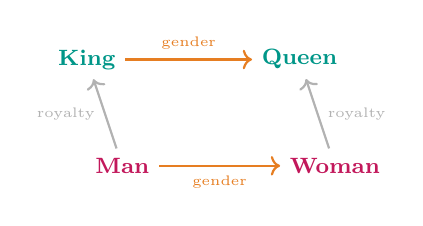
\begin{tikzpicture}[scale=0.9]
        \node[font=\footnotesize\bfseries, linalgTeal] (king) at (0,0) {King};
        \node[font=\footnotesize\bfseries, linalgTeal] (queen) at (3,0) {Queen};
        \node[font=\footnotesize\bfseries, neuronPink] (man) at (0.5,-1.5) {Man};
        \node[font=\footnotesize\bfseries, neuronPink] (woman) at (3.5,-1.5) {Woman};
        \draw[->,thick,accentOrange] (king) -- node[above,font=\tiny]{gender} (queen);
        \draw[->,thick,accentOrange] (man) -- node[below,font=\tiny]{gender} (woman);
        \draw[->,thick,gray!60] (man) -- node[left,font=\tiny]{royalty} (king);
        \draw[->,thick,gray!60] (woman) -- node[right,font=\tiny]{royalty} (queen);
      \end{tikzpicture}

      \vspace{0.1em}
      {\scriptsize Mikolov et al., 2013: Word2Vec}
    \end{column}

    \begin{column}{0.47\textwidth}
      % Interactive callout
      \begin{tcolorbox}[colback=accentOrange!10, colframe=accentOrange,
        fonttitle=\bfseries, title={\faUsers\ Interactive Moment},
        rounded corners, boxrule=1pt, left=3pt, right=3pt, top=2pt, bottom=2pt]
        \centering\large
        $\vec{\text{King}} - \vec{\text{Man}} + \vec{\text{Woman}} = \;?$

        \vspace{0.5em}
        {\small What word do you get?}
      \end{tcolorbox}

      \vspace{0.2em}
      % Embedding pipeline
      \begin{tcolorbox}[colback=gray!5, colframe=gray!40,
        fonttitle=\bfseries\small, title={The Embedding Pipeline},
        rounded corners, boxrule=0.5pt, left=3pt, right=3pt, top=2pt, bottom=2pt]
        \scriptsize
        \texttt{"Hello world"} \\[2pt]
        $\downarrow$ tokenize \\[2pt]
        \texttt{[Hello] [world]} \\[2pt]
        $\downarrow$ embed \\[2pt]
        $\begin{pmatrix}0.2 \\ -0.8 \\ \vdots\end{pmatrix}
         \begin{pmatrix}0.9 \\ 0.1 \\ \vdots\end{pmatrix}$
      \end{tcolorbox}
    \end{column}
  \end{columns}

  \note{
    NOW: When you type ``king'' into an AI, it becomes a list of 768 numbers.
    THEN: 1881, New Haven --- Gibbs formalizes the dot product for physics.
    140 years later, his formula is how your AI knows ``king'' and ``queen'' relate.

    INTERACTIVE MOMENT 1 ($\sim$2 minutes):
    ``What does king minus man plus woman equal?'' Collect guesses.
    Reveal: queen. ``This is not a trick. It's a mathematical property of the space.''
  }
\end{frame}


% ============================================================
% SLIDE 6: Linear Algebra Convergence
% ============================================================
\begin{frame}{Linear Algebra --- The Skeleton Assembled}

  \begin{columns}[T]
    \begin{column}{0.55\textwidth}
      \convergencebar{1}

      \vspace{0.3em}
      \begin{tcolorbox}[colback=linalgTeal!5, colframe=linalgTeal,
        fonttitle=\bfseries\small, title={Section Summary},
        rounded corners, boxrule=0.8pt, left=3pt, right=3pt, top=2pt, bottom=2pt]
        \scriptsize
        \begin{tabular}{@{}ll@{}}
          \toprule
          \textbf{Inventor} & \textbf{Contribution} \\
          \midrule
          Grassmann (1844) & General vector spaces \\
          Sylvester (1850) & Named ``matrix'' \\
          Cayley (1858) & Matrix algebra \\
          Gibbs (1881) & Dot product \\
          Gauss (1809) & Linear systems \\
          Mikolov (2013) & Word embeddings \\
          \bottomrule
        \end{tabular}
      \end{tcolorbox}
    \end{column}

    \begin{column}{0.42\textwidth}
      \begin{insightbox}
        Every layer is a matrix multiplication.

        \vspace{0.2em}
        Every attention score is a dot product.

        \vspace{0.2em}
        The math of the 1840s is the engine of 2026.
      \end{insightbox}

      \vspace{0.3em}
      {\small\itshape One node lit. Nine to go.\\[3pt]
       A skeleton doesn't move.\\
       For that, we need \textbf{calculus} --- the mathematics of change.}
    \end{column}
  \end{columns}

  \note{
    NOW: Node 1 lit --- linear algebra runs inside every AI layer.
    THEN: We jump from the 1840s to an even older story ---
    Archimedes, 250 BCE, Syracuse, computing areas by exhaustion.

    ``One node lit. Nine to go. Now we have the skeleton. But a skeleton
    doesn't move. For that, we need calculus.''
  }
\end{frame}


% ============================================================
% SLIDE 7: Calculus -- The Derivative and Gradient Descent
% ============================================================
\section{Calculus}
\begin{frame}{The Derivative and Gradient Descent}

  \begin{columns}[T]
    \begin{column}{0.52\textwidth}
      % Timeline of calculus
      \begin{tcolorbox}[colback=calculusRed!5, colframe=calculusRed,
        fonttitle=\bfseries\small, title={The Calculus Chain},
        rounded corners, boxrule=0.8pt, left=3pt, right=3pt, top=2pt, bottom=2pt]
        \scriptsize
        \textbf{Archimedes} (c.\,250 BCE) -- method of exhaustion\\[2pt]
        \textbf{Fermat} (1630s) -- tangent lines\\[2pt]
        \textbf{Newton \& Leibniz} (1660s--80s) -- the derivative\\[2pt]
        \textbf{Cauchy} (1847) -- \alert{steepest descent}
      \end{tcolorbox}

      \vspace{0.3em}
      % Gradient descent recipe
      \begin{tcolorbox}[colback=accentOrange!8, colframe=accentOrange,
        fonttitle=\bfseries\small, title={Gradient Descent Recipe},
        rounded corners, boxrule=0.8pt, left=3pt, right=3pt, top=2pt, bottom=2pt]
        \small
        \begin{enumerate}\setlength\itemsep{2pt}
          \item Compute the slope (gradient)
          \item Take a step downhill
          \item Repeat
        \end{enumerate}
        \vspace{2pt}
        \scriptsize $\theta_{\text{new}} = \theta_{\text{old}} - \eta \cdot \nabla L(\theta)$
      \end{tcolorbox}
    \end{column}

    \begin{column}{0.45\textwidth}
      % Loss landscape plot
      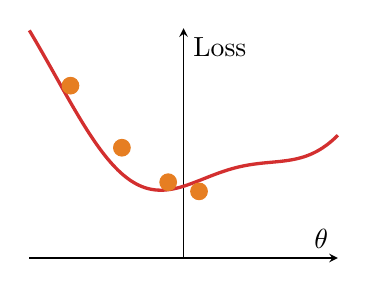
\begin{tikzpicture}
        \begin{axis}[
          width=5.5cm, height=4.5cm,
          domain=-3:3, samples=60,
          axis lines=middle,
          xlabel={$\theta$}, ylabel={Loss},
          ymin=0, ymax=10,
          xtick=\empty, ytick=\empty,
          every axis plot/.append style={no markers},
          clip=false
        ]
          \addplot[calculusRed, very thick, smooth]
            {0.5*(x-0.5)^2 + 0.8*sin(deg(1.5*x)) + 3};
          % Ball positions showing descent
          \addplot[only marks, mark=*, mark size=3pt, accentOrange]
            coordinates {(-2.2,7.5) (-1.2,4.8) (-0.3,3.3) (0.3,2.9)};
        \end{axis}
      \end{tikzpicture}

      \vspace{0.2em}
      {\scriptsize\centering Rolling downhill on the loss landscape.\\
       \emph{Cauchy, 1847.}\par}
    \end{column}
  \end{columns}

  \note{
    NOW: Every time ChatGPT trains on a new sentence, it rolls downhill on a
    mathematical landscape. THEN: 250 BCE --- Archimedes approximates circles
    with polygons. 1847 --- Cauchy asks: ``Can I find the bottom of a valley
    using slopes?'' That question IS how AI learns.

    ``Archimedes was doing proto-calculus. Fermat, Newton, and Leibniz formalized
    the derivative. But the hero for AI is Cauchy, who in 1847 asked: if I can
    compute the slope, can I use it to find the bottom?''
  }
\end{frame}


% ============================================================
% SLIDE 8: Backpropagation -- The Chain Rule Applied
% ============================================================
\begin{frame}{Backpropagation --- The Chain Rule Saves AI}

  \begin{columns}[T]
    \begin{column}{0.48\textwidth}
      \begin{tcolorbox}[colback=calculusRed!5, colframe=calculusRed,
        fonttitle=\bfseries\small, title={The Chain Rule},
        rounded corners, boxrule=0.8pt, left=3pt, right=3pt, top=2pt, bottom=2pt]
        \[
          \frac{df}{dx} = \frac{df}{dg}\cdot\frac{dg}{dx}
        \]
        \small Derivative of a composition\\= product of individual derivatives\\[4pt]
        {\scriptsize Leibniz notation, 1684}
      \end{tcolorbox}

      \vspace{0.3em}
      \begin{tcolorbox}[colback=calculusRed!5, colframe=calculusRed,
        fonttitle=\bfseries\small, title={Timeline},
        rounded corners, boxrule=0.5pt, left=3pt, right=3pt, top=2pt, bottom=2pt]
        \scriptsize
        \textbf{Leibniz} (1684) -- the notation\\[2pt]
        \textbf{Linnainmaa} (1970) -- automatic differentiation\\[2pt]
        \textbf{Rumelhart, Hinton, Williams} (1986) -- backprop in neural nets
      \end{tcolorbox}
    \end{column}

    \begin{column}{0.49\textwidth}
      % Backpropagation diagram
      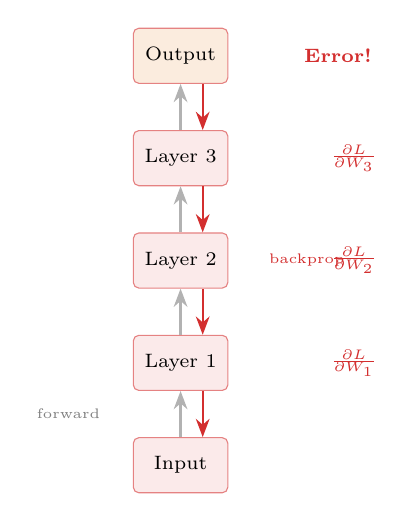
\begin{tikzpicture}[
        layer/.style={draw=calculusRed!60, fill=calculusRed!10,
          minimum width=1.2cm, minimum height=0.7cm, rounded corners=2pt,
          font=\scriptsize},
        >=Stealth
      ]
        \node[layer] (in) at (0,0) {Input};
        \node[layer] (l1) at (0,1.3) {Layer 1};
        \node[layer] (l2) at (0,2.6) {Layer 2};
        \node[layer] (l3) at (0,3.9) {Layer 3};
        \node[layer, fill=accentOrange!15] (out) at (0,5.2) {Output};
        \node[font=\scriptsize\bfseries, calculusRed] at (2,5.2) {Error!};

        % Forward arrows (left)
        \draw[->, thick, gray!60] (in) -- (l1);
        \draw[->, thick, gray!60] (l1) -- (l2);
        \draw[->, thick, gray!60] (l2) -- (l3);
        \draw[->, thick, gray!60] (l3) -- (out);
        \node[font=\tiny, gray, left] at (-0.9,0.65) {forward};

        % Backward arrows (right)
        \draw[<-, thick, calculusRed] ([xshift=8pt]in.north) -- ([xshift=8pt]l1.south);
        \draw[<-, thick, calculusRed] ([xshift=8pt]l1.north) -- ([xshift=8pt]l2.south);
        \draw[<-, thick, calculusRed] ([xshift=8pt]l2.north) -- ([xshift=8pt]l3.south);
        \draw[<-, thick, calculusRed] ([xshift=8pt]l3.north) -- ([xshift=8pt]out.south);
        \node[font=\tiny, calculusRed, right] at (1.0,2.6) {backprop};

        % Gradient labels
        \node[font=\tiny, calculusRed] at (2.2,3.9) {$\frac{\partial L}{\partial W_3}$};
        \node[font=\tiny, calculusRed] at (2.2,2.6) {$\frac{\partial L}{\partial W_2}$};
        \node[font=\tiny, calculusRed] at (2.2,1.3) {$\frac{\partial L}{\partial W_1}$};
      \end{tikzpicture}
    \end{column}
  \end{columns}

  \note{
    NOW: Every AI you use was trained by sending error signals backward through
    96 layers --- that's the chain rule, billions of times.
    THEN: 1684 --- Leibniz publishes the notation. 1970 --- Linnainmaa automates it.
    1986 --- Hinton makes it famous. Three centuries, one idea, powering all of AI.

    ``The chain rule from your calculus class is literally the algorithm that
    trains every AI.''
  }
\end{frame}


% ============================================================
% SLIDE 9: Calculus Convergence
% ============================================================
\begin{frame}{Calculus --- The Learning Engine Assembled}

  \begin{columns}[T]
    \begin{column}{0.55\textwidth}
      \convergencebar{2}

      \vspace{0.3em}
      \begin{tcolorbox}[colback=calculusRed!5, colframe=calculusRed,
        fonttitle=\bfseries\small, title={Section Summary},
        rounded corners, boxrule=0.8pt, left=3pt, right=3pt, top=2pt, bottom=2pt]
        \scriptsize
        \begin{tabular}{@{}ll@{}}
          \toprule
          \textbf{Inventor} & \textbf{Contribution} \\
          \midrule
          Archimedes (c.\,250 BCE) & Proto-calculus \\
          Newton/Leibniz (1680s) & The derivative \\
          Cauchy (1847) & Gradient descent \\
          Linnainmaa (1970) & Auto-differentiation \\
          Hinton et al.\ (1986) & Backprop in NNs \\
          \bottomrule
        \end{tabular}
      \end{tcolorbox}
    \end{column}

    \begin{column}{0.42\textwidth}
      \begin{insightbox}
        Without calculus, you can \emph{build} a neural network but you cannot \emph{train} it.
      \end{insightbox}

      \vspace{0.3em}
      {\small\itshape Two nodes lit.\\[3pt]
       The network has a skeleton and can learn.\\
       But learn \textbf{what}?\\[3pt]
       It learns to predict \textbf{probability distributions} over words.\\
       For that, we need probability theory.}
    \end{column}
  \end{columns}

  \note{
    NOW: Two nodes lit --- linear algebra and calculus run inside every AI.
    THEN: We jump to 1654, Paris --- a gambler writes a letter to Blaise Pascal,
    and probability theory is born.
  }
\end{frame}


% ============================================================
% SLIDE 10: Probability -- From Gambling to Prediction
% ============================================================
\section{Probability}
\begin{frame}{From Gambling to Prediction}

  \begin{columns}[T]
    \begin{column}{0.48\textwidth}
      % Pascal-Fermat exchange with portraits
      \begin{tikzpicture}[
        >=Stealth
      ]
        % Pascal portrait + label
        \node[inner sep=0pt] (pascal_img) at (0,0)
          {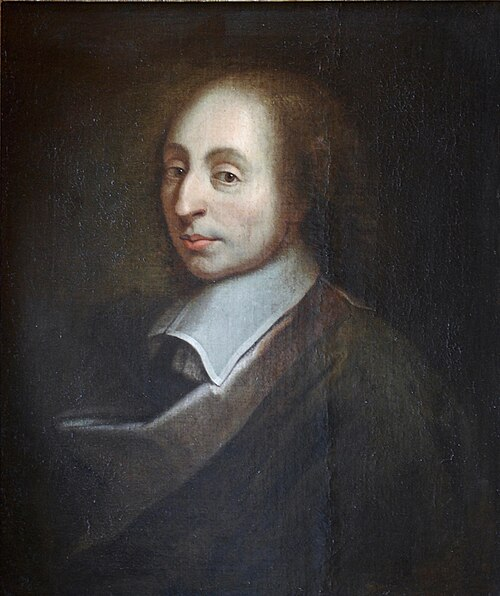
\includegraphics[height=1.2cm,clip]{figures/pascal.jpg}};
        \node[below=1pt of pascal_img, font=\tiny] {Pascal};
        % Fermat portrait + label
        \node[inner sep=0pt] (fermat_img) at (3.2,0)
          {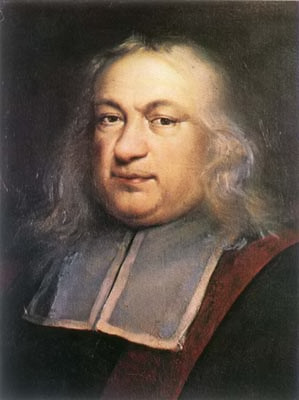
\includegraphics[height=1.2cm,clip]{figures/fermat.jpg}};
        \node[below=1pt of fermat_img, font=\tiny] {Fermat};
        % Exchange arrows
        \draw[->,thick,probBlue!70] ([yshift=2pt]pascal_img.east) --
          node[above,font=\tiny] {1654} ([yshift=2pt]fermat_img.west);
        \draw[<-,thick,probBlue!70] ([yshift=-4pt]pascal_img.east)
          -- ([yshift=-4pt]fermat_img.west);
      \end{tikzpicture}

      \vspace{0.3em}
      % Bayes theorem (no verified portrait exists)
      \begin{tcolorbox}[colback=probBlue!5, colframe=probBlue,
        fonttitle=\bfseries\small,
        title={\tikz[baseline=-0.5ex]{\node[draw=probBlue,fill=probBlue!15,
          circle,inner sep=1pt,font=\scriptsize\bfseries]{?};}
          ~Bayes (1763)},
        rounded corners, boxrule=0.5pt, left=3pt, right=3pt, top=2pt, bottom=2pt]
        \small
        $P(A \mid B) = \dfrac{P(B \mid A)\, P(A)}{P(B)}$\\[4pt]
        \scriptsize Update beliefs from evidence.\\
        LLMs learn: $P(\text{next word} \mid \text{context})$
      \end{tcolorbox}
    \end{column}

    \begin{column}{0.49\textwidth}
      % Shannon's language model with portrait
      \begin{tcolorbox}[colback=infoAmber!8, colframe=infoAmber,
        fonttitle=\bfseries\small,
        title={\raisebox{-0.4em}{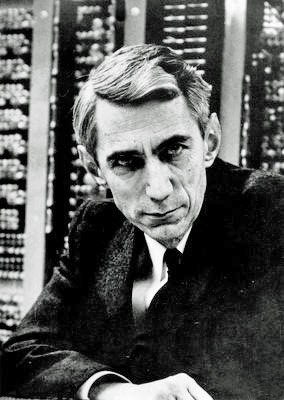
\includegraphics[height=1cm,clip]{figures/shannon.jpg}}%
          ~Shannon (1948)},
        rounded corners, boxrule=0.5pt, left=3pt, right=3pt, top=2pt, bottom=2pt]
        \scriptsize
        \textbf{0th order:} XFOML RXKHRJFFJUJ\\[2pt]
        \textbf{1st order:} OCRO HLI RGWR\\[2pt]
        \textbf{2nd order:} ON IE ANTSOUTINYS\\[2pt]
        \textbf{Word bigram:} THE HEAD AND IN FRONTAL\\[4pt]
        More context $=$ more readable.\\
        This IS what every LLM does.
      \end{tcolorbox}

      \vspace{0.3em}
      \begin{llmconnection}
        \scriptsize
        Every word your AI generates is chosen by probability ---
        a distribution over 50,000+ possible next tokens.
      \end{llmconnection}
    \end{column}
  \end{columns}

  \note{
    NOW: Every word your AI generates is chosen by probability. THEN: 1654 ---
    the Chevalier de M\'er\'e loses at dice and writes to Pascal. That letter
    launched the mathematics that decides every word an AI says.

    ``Probability was born because a gambler asked how to split a pot.
    Two centuries later, Bayes showed how to update beliefs from evidence.
    Then Shannon modeled English as a statistical process. That's exactly
    what every LLM does.''
  }
\end{frame}


% ============================================================
% SLIDE 11: Softmax -- INTERACTIVE
% ============================================================
\begin{frame}{Softmax --- From Thermodynamics to Token Prediction}

  \begin{columns}[T]
    \begin{column}{0.48\textwidth}
      \begin{tcolorbox}[colback=probBlue!5, colframe=probBlue,
        fonttitle=\bfseries\small, title={Boltzmann (1870s)},
        rounded corners, boxrule=0.8pt, left=3pt, right=3pt, top=2pt, bottom=2pt]
        \small Energy distribution of gas molecules:\\[4pt]
        $\displaystyle\text{softmax}(z_i) = \frac{e^{z_i}}{\sum_j e^{z_j}}$\\[6pt]
        \scriptsize Same formula. Now picks words.
      \end{tcolorbox}

      \vspace{0.3em}
      % Softmax pipeline
      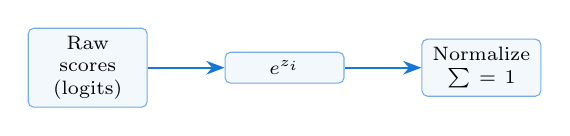
\begin{tikzpicture}[
        box/.style={draw=probBlue!60, fill=probBlue!5, rounded corners=2pt,
          font=\scriptsize, inner sep=3pt, minimum width=1.5cm,
          text width=1.3cm, align=center},
        >=Stealth
      ]
        \node[box] (logits) at (0,0) {Raw scores (logits)};
        \node[box] (exp) at (2.5,0) {$e^{z_i}$};
        \node[box] (norm) at (5,0) {Normalize $\sum = 1$};
        \draw[->,thick,probBlue] (logits) -- (exp);
        \draw[->,thick,probBlue] (exp) -- (norm);
      \end{tikzpicture}
    \end{column}

    \begin{column}{0.49\textwidth}
      % Interactive moment
      \begin{tcolorbox}[colback=accentOrange!10, colframe=accentOrange,
        fonttitle=\bfseries, title={\faUsers\ Interactive Moment},
        rounded corners, boxrule=1pt, left=3pt, right=3pt, top=3pt, bottom=3pt]
        \centering
        {\large ``The cat sat on the \rule{1.5cm}{0.4pt}''}

        \vspace{0.3em}
        {\small What word comes next?}
      \end{tcolorbox}

      \vspace{0.3em}
      % Bar chart of probabilities (manual TikZ bars)
      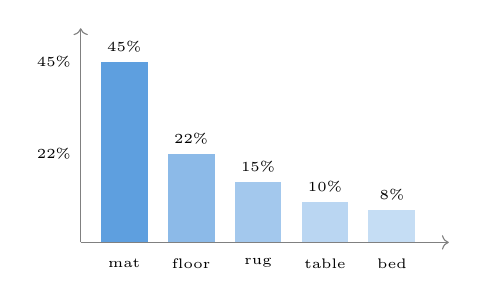
\begin{tikzpicture}[scale=0.85]
        % Axis
        \draw[->,gray] (0,0) -- (5.5,0);
        \draw[->,gray] (0,0) -- (0,3.2);
        \node[font=\tiny,left] at (0,2.7) {45\%};
        \node[font=\tiny,left] at (0,1.32) {22\%};
        % Bars
        \fill[probBlue!70] (0.3,0) rectangle (1,2.7);
        \node[font=\tiny,below] at (0.65,-0.1) {mat};
        \fill[probBlue!50] (1.3,0) rectangle (2,1.32);
        \node[font=\tiny,below] at (1.65,-0.1) {floor};
        \fill[probBlue!40] (2.3,0) rectangle (3,0.9);
        \node[font=\tiny,below] at (2.65,-0.1) {rug};
        \fill[probBlue!30] (3.3,0) rectangle (4,0.6);
        \node[font=\tiny,below] at (3.65,-0.1) {table};
        \fill[probBlue!25] (4.3,0) rectangle (5,0.48);
        \node[font=\tiny,below] at (4.65,-0.1) {bed};
        % Labels on bars
        \node[font=\tiny,above] at (0.65,2.7) {45\%};
        \node[font=\tiny,above] at (1.65,1.32) {22\%};
        \node[font=\tiny,above] at (2.65,0.9) {15\%};
        \node[font=\tiny,above] at (3.65,0.6) {10\%};
        \node[font=\tiny,above] at (4.65,0.48) {8\%};
      \end{tikzpicture}
    \end{column}
  \end{columns}

  \note{
    NOW: Every single word your AI says is chosen by this formula --- softmax.
    THEN: 1870s, Vienna --- Ludwig Boltzmann is studying how gas molecules
    distribute among energy levels. He writes $e^x / \sum e^x$. That exact formula
    now picks every word an AI says.

    INTERACTIVE MOMENT 2 ($\sim$2 minutes): Quick poll. ``The cat sat on the
    \underline{\hspace{1cm}}.'' Collect answers. Show the AI's softmax distribution.
  }
\end{frame}


% ============================================================
% SLIDE 12: Probability + Info Theory Convergence
% ============================================================
\begin{frame}{Cross-Entropy --- Measuring How Wrong the AI Is}

  \begin{columns}[T]
    \begin{column}{0.52\textwidth}
      \convergencebar{4}

      \vspace{0.3em}
      \begin{tcolorbox}[colback=infoAmber!8, colframe=infoAmber,
        fonttitle=\bfseries\small, title={Shannon's Loss Function (1948)},
        rounded corners, boxrule=0.8pt, left=3pt, right=3pt, top=2pt, bottom=2pt]
        \small
        Cross-entropy loss $= -\log\bigl(p(\text{correct word})\bigr)$\\[6pt]
        \scriptsize
        \begin{tabular}{@{}lcc@{}}
          & \textbf{Confidence} & \textbf{Loss}\\
          \midrule
          ``mat'' at 30\% & 0.30 & 1.20\\
          ``mat'' at 80\% & 0.80 & 0.22\\
        \end{tabular}\\[6pt]
        Training = minimizing cross-entropy\\
        = making the model more confident\\about the RIGHT word.
      \end{tcolorbox}
    \end{column}

    \begin{column}{0.45\textwidth}
      \begin{insightbox}
        \small
        Shannon's 1948 paper contributes to \textbf{two} building blocks:
        language modeling (probability) AND the loss function (information theory).
      \end{insightbox}

      \vspace{0.3em}
      {\small\itshape Four nodes lit.\\[4pt]
       Prediction math: \textcolor{probBlue}{probability}\\
       Scoring math: \textcolor{infoAmber}{information theory}\\
       Learning math: \textcolor{calculusRed}{calculus}\\
       Structure math: \textcolor{linalgTeal}{linear algebra}\\[6pt]
       But we need something to \textbf{run it on}.}
    \end{column}
  \end{columns}

  \note{
    NOW: Every AI checks its own mistakes using ``cross-entropy loss.''
    THEN: 1948, Bell Labs --- Claude Shannon publishes ``A Mathematical Theory
    of Communication.'' He needed a way to measure information. That measure IS
    the loss function that trains every LLM.

    ``Shannon's paper is so foundational it contributes to two sections.
    He modeled language statistically AND created the measure for how good
    that model is.''
  }
\end{frame}


% ============================================================
% SLIDE 13: Logic & Computation
% ============================================================
\section{Logic \& Computation}
\begin{frame}{Logic \& Computation --- The Substrate}

  \begin{columns}[T]
    \begin{column}{0.48\textwidth}
      \begin{tcolorbox}[colback=logicGray!5, colframe=logicGray,
        fonttitle=\bfseries\small, title={The Logic Chain},
        rounded corners, boxrule=0.8pt, left=3pt, right=3pt, top=2pt, bottom=2pt]
        \scriptsize
        \textbf{Boole} (1854) --- Logic as algebra.\\
        True/false $=$ 1/0. Son of a shoemaker.\\[2pt]
        \textbf{Turing} (1936) --- Universal machine.\\
        Can compute anything computable.\\[2pt]
        \textbf{Von Neumann} (1945) --- Stored program.\\
        The architecture of every computer.\\[2pt]
        \textbf{NVIDIA CUDA} (2007) --- GPUs.\\
        Billions of parallel operations.
      \end{tcolorbox}

      \vspace{0.3em}
      % Boolean gates
      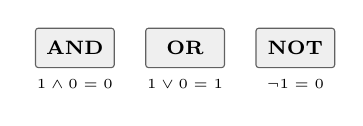
\begin{tikzpicture}[scale=0.7,
        gate/.style={draw=logicGray, fill=logicGray!10, minimum width=1cm,
          minimum height=0.5cm, rounded corners=1pt, font=\scriptsize\bfseries}
      ]
        \node[gate] (and) at (0,0) {AND};
        \node[gate] (or) at (2,0) {OR};
        \node[gate] (not) at (4,0) {NOT};
        \node[font=\tiny,below] at (0,-0.4) {$1 \wedge 0 = 0$};
        \node[font=\tiny,below] at (2,-0.4) {$1 \vee 0 = 1$};
        \node[font=\tiny,below] at (4,-0.4) {$\neg 1 = 0$};
      \end{tikzpicture}
    \end{column}

    \begin{column}{0.49\textwidth}
      % The paradox
      \begin{tcolorbox}[colback=aiViolet!8, colframe=aiViolet,
        fonttitle=\bfseries\small, title={The Paradox},
        rounded corners, boxrule=0.8pt, left=3pt, right=3pt, top=2pt, bottom=2pt]
        \small
        G\"odel and Turing proved that no formal system can capture all truth.

        \vspace{0.15em}
        Yet neural networks --- running on the hardware that logic built ---
        learned to do things formal logic cannot:

        \vspace{0.1em}
        \centering
        \textbf{translate, write poetry, reason by analogy.}

        \vspace{0.15em}
        \raggedright
        \scriptsize The machines that logic built transcended the limitations
        that logic discovered.
      \end{tcolorbox}

      \vspace{0.1em}
      {\tiny\itshape ``Boole was a self-taught son of a shoemaker who reduced
       logic to algebra. Turing imagined a machine that could compute anything
       computable. Their ideas ARE the hardware your AI runs on.''}
    \end{column}
  \end{columns}

  \note{
    NOW: The AI on your phone processes billions of Boolean operations per second.
    THEN: 1854, Cork --- Boole reduces logic to algebra. 1936, Cambridge ---
    Turing imagines a universal machine. Their ideas ARE the hardware.

    ``Here's the paradox: logicians dreamed of mechanical thought.
    They proved it was impossible in general. Then neural networks did it anyway.''
  }
\end{frame}


% ============================================================
% SLIDE 14: Function Approximation + Convergence (5-6 lit)
% ============================================================
\begin{frame}{Function Approximation --- The Guarantee}

  \begin{columns}[T]
    \begin{column}{0.5\textwidth}
      \convergencebar{6}

      \vspace{0.1em}
      % Fourier series plot
      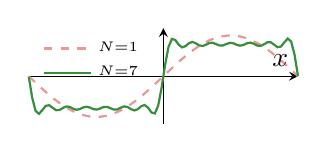
\begin{tikzpicture}
        \begin{axis}[
          width=5cm, height=2.8cm,
          domain=-3.14:3.14, samples=80,
          axis lines=middle,
          xlabel={$x$}, ylabel={},
          ymin=-1.5, ymax=1.5,
          xtick=\empty, ytick=\empty,
          legend style={at={(0.02,0.98)},anchor=north west,
            font=\tiny, draw=none, fill=none},
          every axis plot/.append style={thick, no markers},
          clip=false
        ]
          \addplot[calculusRed!50, dashed]
            {(4/3.14159)*sin(deg(x))};
          \addlegendentry{$N{=}1$}
          \addplot[approxGreen, thick]
            {(4/3.14159)*(sin(deg(x))
             + sin(deg(3*x))/3
             + sin(deg(5*x))/5
             + sin(deg(7*x))/7
             + sin(deg(9*x))/9
             + sin(deg(11*x))/11
             + sin(deg(13*x))/13)};
          \addlegendentry{$N{=}7$}
        \end{axis}
      \end{tikzpicture}%
      {\scriptsize\centering Any function $=$ sum of waves. \emph{Fourier, 1807.}\par}
    \end{column}

    \begin{column}{0.47\textwidth}
      \begin{tcolorbox}[colback=approxGreen!5, colframe=approxGreen,
        fonttitle=\bfseries\small, title={The Chain of Guarantees},
        rounded corners, boxrule=0.8pt, left=3pt, right=3pt, top=1pt, bottom=1pt]
        \scriptsize
        \textbf{Fourier} (1807)\\
        Any function as a sum of sines.\\[2pt]
        \textbf{Weierstrass} (1885)\\
        Polynomials can approximate anything.\\[2pt]
        \textbf{Cybenko} (1989)\\
        Neural networks can approximate \emph{any} continuous function.
      \end{tcolorbox}

      \vspace{0.1em}
      \begin{tcolorbox}[colback=aiViolet!8,colframe=aiViolet!60,
        boxrule=0.5pt,rounded corners,left=3pt,right=3pt,top=1pt,bottom=1pt]
        \small A neural network \textbf{can} learn any continuous function.
        This is not an analogy. It is a \emph{mathematical theorem}.
      \end{tcolorbox}

      \vspace{0.1em}
      {\small\itshape Six nodes lit. We know they CAN learn anything.\\
       But what IS a neural network?}
    \end{column}
  \end{columns}

  \note{
    NOW: The reason anyone believes neural networks can learn language, vision,
    reasoning is a theorem from 1989. THEN: 1807 --- Fourier claims any function
    is a sum of sines. 1989 --- Cybenko proves the same for neural networks.
    The guarantee that makes all of AI possible.

    ``Fourier wanted to solve the heat equation. A century later, Cybenko proved
    the same thing for neural networks. This theorem is why people bet on NNs.''
  }
\end{frame}


% ============================================================
% SLIDE 15: The Artificial Neuron
% ============================================================
\section{The Neuron \& Depth}
\begin{frame}{The Neuron --- From Biology to Mathematics}

  \begin{columns}[T]
    \begin{column}{0.48\textwidth}
      \begin{tcolorbox}[colback=neuronPink!5, colframe=neuronPink,
        fonttitle=\bfseries\small, title={McCulloch \& Pitts (1943)},
        rounded corners, boxrule=0.8pt, left=3pt, right=3pt, top=2pt, bottom=2pt]
        \scriptsize
        A neurophysiologist and a \textbf{teenage runaway}
        (self-taught logician, no degree) created the mathematical neuron.
      \end{tcolorbox}

      \vspace{0.2em}
      % McCulloch-Pitts neuron diagram
      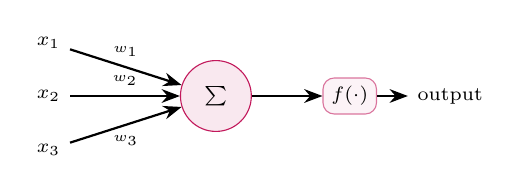
\begin{tikzpicture}[
        >=Stealth, scale=0.85
      ]
        \node[circle, draw=neuronPink, fill=neuronPink!10,
          minimum size=0.9cm, font=\scriptsize] (n) at (2.5,0) {$\sum$};
        % Inputs
        \node[font=\scriptsize] (x1) at (0,0.8) {$x_1$};
        \node[font=\scriptsize] (x2) at (0,0) {$x_2$};
        \node[font=\scriptsize] (x3) at (0,-0.8) {$x_3$};
        \draw[->, thick] (x1) -- node[above,font=\tiny]{$w_1$} (n);
        \draw[->, thick] (x2) -- node[above,font=\tiny]{$w_2$} (n);
        \draw[->, thick] (x3) -- node[below,font=\tiny]{$w_3$} (n);
        % Output
        \node[draw=neuronPink!60, fill=neuronPink!5, rounded corners,
          font=\scriptsize, inner sep=3pt] (f) at (4.5,0) {$f(\cdot)$};
        \draw[->, thick] (n) -- (f);
        \node[font=\scriptsize] (y) at (6,0) {output};
        \draw[->, thick] (f) -- (y);
      \end{tikzpicture}
    \end{column}

    \begin{column}{0.49\textwidth}
      \begin{tcolorbox}[colback=neuronPink!5, colframe=neuronPink,
        fonttitle=\bfseries\small, title={Rosenblatt's Perceptron (1958)},
        rounded corners, boxrule=0.8pt, left=3pt, right=3pt, top=2pt, bottom=2pt]
        \scriptsize
        A room-sized machine with 400 photocells that could \textbf{learn}.

        \vspace{0.2em}
        The New York Times: ``a machine that could walk, talk, see, write\ldots''

        \vspace{0.3em}
        \centering
        The hype was enormous.

        \vspace{0.2em}
        \textbf{And then came the crash.}
      \end{tcolorbox}

      \vspace{0.3em}
      % Learning loop
      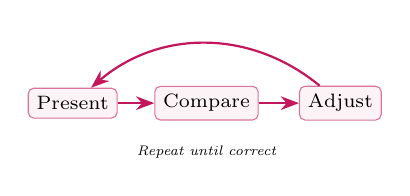
\begin{tikzpicture}[
        box/.style={draw=neuronPink!60, fill=neuronPink!5, rounded corners=2pt,
          font=\scriptsize, inner sep=3pt},
        >=Stealth, scale=0.85
      ]
        \node[box] (present) at (0,0) {Present};
        \node[box] (compare) at (2,0) {Compare};
        \node[box] (adjust) at (4,0) {Adjust};
        \draw[->,thick,neuronPink] (present) -- (compare);
        \draw[->,thick,neuronPink] (compare) -- (adjust);
        \draw[->,thick,neuronPink] (adjust) to[bend right=40] (present);
        \node[font=\tiny\itshape, below] at (2,-0.5) {Repeat until correct};
      \end{tikzpicture}
    \end{column}
  \end{columns}

  \note{
    NOW: Every AI is built from billions of artificial neurons. THEN: 1943,
    Chicago --- McCulloch and Pitts write the paper. 1958, Cornell ---
    Rosenblatt builds a machine that can learn. The press goes wild.
    And then it all collapses.

    ``McCulloch was in his 40s. Pitts was about 20 and had no degree. Their
    paper launched neural network research. Then Rosenblatt built the Perceptron.
    The hype was enormous. And then came the crash.''
  }
\end{frame}


% ============================================================
% SLIDE 16: The XOR Crash and AI Winter
% ============================================================
\begin{frame}{The Crash and Comeback}

  \begin{columns}[T]
    \begin{column}{0.45\textwidth}
      % XOR problem
      \begin{tcolorbox}[colback=calculusRed!5, colframe=calculusRed,
        fonttitle=\bfseries\small, title={The XOR Problem (1969)},
        rounded corners, boxrule=0.8pt, left=3pt, right=3pt, top=2pt, bottom=2pt]
        \centering
        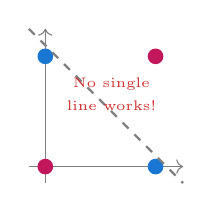
\begin{tikzpicture}[scale=0.7]
          \draw[->,gray,thin] (-0.3,0)--(2.5,0);
          \draw[->,gray,thin] (0,-0.3)--(0,2.5);
          \node[circle,fill=neuronPink,inner sep=2pt] at (0,0) {};
          \node[circle,fill=neuronPink,inner sep=2pt] at (2,2) {};
          \node[circle,fill=probBlue,inner sep=2pt] at (2,0) {};
          \node[circle,fill=probBlue,inner sep=2pt] at (0,2) {};
          \draw[dashed,gray,thick] (-0.3,2.5) -- (2.5,-0.3);
          \node[font=\tiny,text=calculusRed] at (1.2,1.5) {No single};
          \node[font=\tiny,text=calculusRed] at (1.2,1.1) {line works!};
        \end{tikzpicture}

        \vspace{0.2em}
        \scriptsize Minsky \& Papert proved:\\
        one layer cannot learn XOR.
      \end{tcolorbox}
    \end{column}

    \begin{column}{0.52\textwidth}
      % AI winter timeline
      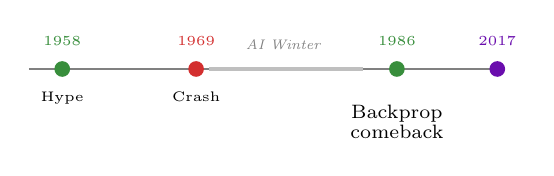
\begin{tikzpicture}[scale=0.85]
        % Timeline
        \draw[thick,gray] (0,0) -- (7,0);
        % Hype
        \node[circle,fill=approxGreen,inner sep=2pt] (h) at (0.5,0) {};
        \node[font=\tiny,above,text=approxGreen] at (0.5,0.2) {1958};
        \node[font=\tiny,below] at (0.5,-0.2) {Hype};
        % Crash
        \node[circle,fill=calculusRed,inner sep=2pt] (c) at (2.5,0) {};
        \node[font=\tiny,above,text=calculusRed] at (2.5,0.2) {1969};
        \node[font=\tiny,below] at (2.5,-0.2) {Crash};
        % Winter
        \draw[very thick, gray!50] (2.7,0) -- (5,0);
        \node[font=\tiny\itshape, above, text=gray] at (3.8,0.15) {AI Winter};
        % Comeback
        \node[circle,fill=approxGreen,inner sep=2pt] (r) at (5.5,0) {};
        \node[font=\tiny,above,text=approxGreen] at (5.5,0.2) {1986};
        \node[font=\tiny,below,text width=1.5cm,align=center] at (5.5,-0.4) {\scriptsize Backprop\\comeback};
        % Modern
        \node[circle,fill=aiViolet,inner sep=2pt] (m) at (7,0) {};
        \node[font=\tiny,above,text=aiViolet] at (7,0.2) {2017};
      \end{tikzpicture}

      \vspace{0.5em}
      \begin{tcolorbox}[colback=approxGreen!8, colframe=approxGreen,
        fonttitle=\bfseries\small, title={The Solution: More Layers},
        rounded corners, boxrule=0.8pt, left=3pt, right=3pt, top=2pt, bottom=2pt]
        \scriptsize
        Minsky \& Papert's math was correct.\\
        Their conclusion was wrong.\\[3pt]
        The solution: \textbf{add more layers.}\\[3pt]
        Rumelhart, Hinton \& Williams (1986):\\
        backpropagation can train multi-layer networks.\\[3pt]
        \textbf{The chain rule saved an entire research program.}
      \end{tcolorbox}
    \end{column}
  \end{columns}

  \note{
    NOW: Modern AI uses networks with 96+ layers. THEN: 1969 ---
    Minsky and Papert prove one layer is not enough and the field dies
    for 17 years. 1986 --- Hinton shows that with the chain rule you can
    train MANY layers. The comeback that made your AI possible.

    ``It took 17 years. The AI winter was caused by stopping one layer too soon.''
  }
\end{frame}


% ============================================================
% SLIDE 17: Depth -- Activation, Residuals, Normalization
% ============================================================
\begin{frame}{Depth --- Activation, Residuals, Normalization}

  \begin{columns}[T]
    \begin{column}{0.33\textwidth}
      % Activation functions
      \begin{tcolorbox}[colback=neuronPink!5, colframe=neuronPink,
        fonttitle=\bfseries\scriptsize, title={Activation},
        rounded corners, boxrule=0.5pt, left=2pt, right=2pt, top=2pt, bottom=2pt]
        \centering
        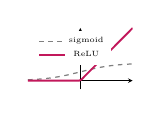
\begin{tikzpicture}[scale=0.55]
          \begin{axis}[
            width=4cm, height=3cm,
            domain=-3:3, samples=50,
            axis lines=middle,
            xtick=\empty, ytick=\empty,
            ymin=-0.5, ymax=3,
            every axis plot/.append style={thick, no markers},
            legend style={at={(0.05,0.95)},anchor=north west,
              font=\tiny, draw=none}
          ]
            \addplot[gray, dashed] {1/(1+exp(-x))};
            \addlegendentry{sigmoid}
            \addplot[neuronPink, very thick] {max(0,x)};
            \addlegendentry{ReLU}
          \end{axis}
        \end{tikzpicture}

        \vspace{0.1em}
        \scriptsize Without this,\\100 layers = 1 layer.
      \end{tcolorbox}
    \end{column}

    \begin{column}{0.33\textwidth}
      % Residual connections
      \begin{tcolorbox}[colback=neuronPink!5, colframe=neuronPink,
        fonttitle=\bfseries\scriptsize, title={Residuals (He, 2015)},
        rounded corners, boxrule=0.5pt, left=2pt, right=2pt, top=2pt, bottom=2pt]
        \centering
        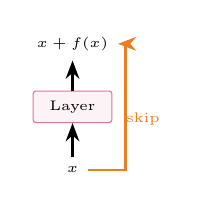
\begin{tikzpicture}[scale=0.8,
          box/.style={draw=neuronPink!60, fill=neuronPink!5,
            minimum width=1cm, minimum height=0.4cm, font=\tiny,
            rounded corners=1pt},
          >=Stealth
        ]
          \node[box] (layer) at (0,0) {Layer};
          \node[font=\tiny] (x) at (0,-1) {$x$};
          \node[font=\tiny] (out) at (0,1) {$x + f(x)$};
          \draw[->,thick] (x) -- (layer);
          \draw[->,thick] (layer) -- (out);
          \draw[->,thick,accentOrange] (x.east) -- ++(0.6,0) |- (out.east);
          \node[font=\tiny,accentOrange,right] at (0.7,-0.2) {skip};
        \end{tikzpicture}

        \vspace{0.1em}
        \scriptsize Signal doesn't fade.
      \end{tcolorbox}
    \end{column}

    \begin{column}{0.33\textwidth}
      % Layer normalization
      \begin{tcolorbox}[colback=neuronPink!5, colframe=neuronPink,
        fonttitle=\bfseries\scriptsize, title={LayerNorm (Ba, 2016)},
        rounded corners, boxrule=0.5pt, left=2pt, right=2pt, top=2pt, bottom=2pt]
        \centering
        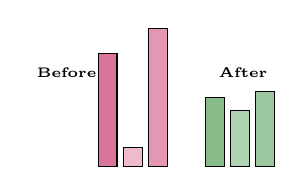
\begin{tikzpicture}[scale=0.8]
          % Before
          \node[font=\tiny\bfseries] at (-0.5,1.5) {Before};
          \draw[fill=neuronPink!60] (0,0) rectangle (0.3,1.8);
          \draw[fill=neuronPink!30] (0.4,0) rectangle (0.7,0.3);
          \draw[fill=neuronPink!45] (0.8,0) rectangle (1.1,2.2);
          % After
          \node[font=\tiny\bfseries] at (2.3,1.5) {After};
          \draw[fill=approxGreen!60] (1.7,0) rectangle (2.0,1.1);
          \draw[fill=approxGreen!40] (2.1,0) rectangle (2.4,0.9);
          \draw[fill=approxGreen!50] (2.5,0) rectangle (2.8,1.2);
        \end{tikzpicture}

        \vspace{0.1em}
        \scriptsize Numbers don't explode.
      \end{tcolorbox}
    \end{column}
  \end{columns}

  \vspace{0.3em}
  \begin{center}
    \begin{tcolorbox}[colback=aiViolet!8, colframe=aiViolet,
      boxrule=0.5pt, rounded corners, width=0.85\textwidth,
      left=4pt, right=4pt, top=2pt, bottom=2pt]
      \centering\small
      \textbf{``Add \& Norm''} in the transformer = He's residual + Ba's normalization.\\
      You will see them on slide 23.
    \end{tcolorbox}
  \end{center}

  \note{
    NOW: The ``Add \& Norm'' blocks inside every transformer layer.
    THEN: 2015, Microsoft Research Beijing --- He adds skip connections.
    2016, Toronto --- Ba adds normalization. Two quiet papers that made
    96-layer networks possible.

    ``Three inventions. Activation adds nonlinearity. Residuals preserve the
    signal. Normalization keeps everything stable. Invisible to the user,
    essential to the machine.''
  }
\end{frame}


% ============================================================
% SLIDE 18: Neuron Convergence
% ============================================================
\begin{frame}{The Neuron \& Depth --- Seven Nodes Lit}

  \begin{columns}[T]
    \begin{column}{0.55\textwidth}
      \convergencebar{7}

      \vspace{0.3em}
      \begin{tcolorbox}[colback=neuronPink!5, colframe=neuronPink,
        fonttitle=\bfseries\small, title={Section Summary},
        rounded corners, boxrule=0.8pt, left=3pt, right=3pt, top=2pt, bottom=2pt]
        \scriptsize
        \begin{tabular}{@{}ll@{}}
          \toprule
          \textbf{Inventor} & \textbf{Contribution} \\
          \midrule
          McCulloch \& Pitts (1943) & Mathematical neuron \\
          Rosenblatt (1958) & Perceptron (learning) \\
          Minsky \& Papert (1969) & XOR impossibility \\
          Hinton et al.\ (1986) & Backprop revival \\
          Nair \& Hinton (2010) & ReLU activation \\
          He et al.\ (2015) & Residual connections \\
          Ba et al.\ (2016) & Layer normalization \\
          \bottomrule
        \end{tabular}
      \end{tcolorbox}
    \end{column}

    \begin{column}{0.42\textwidth}
      \begin{insightbox}
        \small
        Billions of neurons, stacked 96+ layers deep, with activation, residuals,
        and normalization.

        \vspace{0.3em}
        But language is \textbf{sequential}.\\
        ``Dog bites man'' $\neq$ ``Man bites dog.''
      \end{insightbox}

      \vspace{0.3em}
      {\small\itshape Seven nodes lit.\\[3pt]
       We can build neurons, stack them deep, and train them.\\[3pt]
       But how do you process a \textbf{sequence}?}
    \end{column}
  \end{columns}

  \note{
    NOW: Seven of ten nodes lit --- the AI has neurons, depth, and can learn.
    But it cannot yet read a sentence in order.
    THEN: We jump to 1906, St.\ Petersburg --- Andrey Markov is analyzing
    the poetry of Pushkin, and he invents sequence modeling.

    ``Language is sequential. Word order matters. How do you process a sequence?
    That took another set of inventions.''
  }
\end{frame}


% ============================================================
% SLIDE 19: Sequence Modeling -- Markov to Attention
% ============================================================
\section{Sequence Modeling}
\begin{frame}{From Markov Chains to Attention}

  \begin{columns}[T]
    \begin{column}{0.48\textwidth}
      % Markov chain
      \begin{tcolorbox}[colback=seqIndigo!5, colframe=seqIndigo,
        fonttitle=\bfseries\small, title={Markov (1906)},
        rounded corners, boxrule=0.8pt, left=3pt, right=3pt, top=2pt, bottom=2pt]
        \centering
        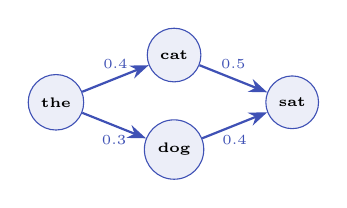
\begin{tikzpicture}[scale=0.75,
          state/.style={circle, draw=seqIndigo, fill=seqIndigo!10,
            minimum size=0.6cm, font=\tiny\bfseries},
          >=Stealth
        ]
          \node[state] (a) at (0,0) {the};
          \node[state] (b) at (2,0.8) {cat};
          \node[state] (c) at (2,-0.8) {dog};
          \node[state] (d) at (4,0) {sat};
          \draw[->,thick,seqIndigo] (a) -- node[above,font=\tiny]{0.4} (b);
          \draw[->,thick,seqIndigo] (a) -- node[below,font=\tiny]{0.3} (c);
          \draw[->,thick,seqIndigo] (b) -- node[above,font=\tiny]{0.5} (d);
          \draw[->,thick,seqIndigo] (c) -- node[below,font=\tiny]{0.4} (d);
        \end{tikzpicture}

        \vspace{0.2em}
        \scriptsize Analyzed Pushkin's poetry.\\
        Next word depends only on current word.
      \end{tcolorbox}

      \vspace{0.2em}
      % RNN problem
      \begin{tcolorbox}[colback=calculusRed!5, colframe=calculusRed,
        fonttitle=\bfseries\scriptsize, title={The Problem: Memory Fades},
        rounded corners, boxrule=0.5pt, left=3pt, right=3pt, top=2pt, bottom=2pt]
        \scriptsize
        RNNs: memory fades after $\sim$50 words.\\
        The beginning of a paragraph is forgotten.
      \end{tcolorbox}
    \end{column}

    \begin{column}{0.49\textwidth}
      % Attention breakthrough
      \begin{tcolorbox}[colback=seqIndigo!5, colframe=seqIndigo,
        fonttitle=\bfseries\small,
        title={Attention (Bahdanau, 2014)},
        rounded corners, boxrule=1pt, left=3pt, right=3pt, top=3pt, bottom=3pt]
        \small
        Instead of compressing everything into one vector,
        \textbf{look back at the whole input.}

        \vspace{0.3em}
        \centering
        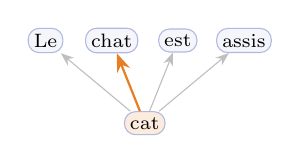
\begin{tikzpicture}[scale=0.7,
          word/.style={draw=seqIndigo!40, fill=seqIndigo!5, rounded corners,
            font=\scriptsize, inner sep=2pt},
          >=Stealth
        ]
          \node[word] (w1) at (0,0) {Le};
          \node[word] (w2) at (1.2,0) {chat};
          \node[word] (w3) at (2.4,0) {est};
          \node[word] (w4) at (3.6,0) {assis};
          \node[word, fill=accentOrange!15] (t) at (1.8,-1.5) {cat};
          \draw[->,thick,accentOrange] (t) -- (w2);
          \draw[->,thin,gray!50] (t) -- (w1);
          \draw[->,thin,gray!50] (t) -- (w3);
          \draw[->,thin,gray!50] (t) -- (w4);
        \end{tikzpicture}

        \vspace{0.2em}
        \scriptsize The model \textbf{chooses} what to attend to.
      \end{tcolorbox}

      \vspace{0.2em}
      {\scriptsize\itshape Without this 2014 paper, there would be no GPT, no Claude.}
    \end{column}
  \end{columns}

  \note{
    NOW: Your AI can read a 100,000-word document and remember the first sentence.
    That is attention. THEN: 1906 --- Markov analyzes Pushkin's poetry.
    2014 --- Bahdanau asks: ``Why forget anything?'' and invents attention.

    ``Markov chains have a fatal flaw: memory fades. Bahdanau asked a simple
    question: why compress everything into one vector when you can look back
    at the whole input? That's attention.''
  }
\end{frame}


% ============================================================
% SLIDE 20: Attention -- The Bridge to the Transformer
% ============================================================
\begin{frame}{Attention --- The Bridge to the Transformer}

  \begin{columns}[T]
    \begin{column}{0.55\textwidth}
      \convergencebar{8}

      \vspace{0.3em}
      \begin{tcolorbox}[colback=seqIndigo!5, colframe=seqIndigo,
        fonttitle=\bfseries\small, title={Eight Nodes Lit},
        rounded corners, boxrule=0.8pt, left=3pt, right=3pt, top=2pt, bottom=2pt]
        \small
        Two thousand years of mathematics.\\[4pt]
        \textcolor{linalgTeal}{Linear algebra},
        \textcolor{calculusRed}{calculus},
        \textcolor{probBlue}{probability},
        \textcolor{infoAmber}{information theory},
        \textcolor{logicGray}{logic},
        \textcolor{approxGreen}{function approximation},
        \textcolor{neuronPink}{the neuron},
        \textcolor{seqIndigo}{sequences}.\\[6pt]
        All of these streams are about to converge in a single architecture.
      \end{tcolorbox}
    \end{column}

    \begin{column}{0.42\textwidth}
      \vspace{1em}
      \begin{center}
        {\Large\bfseries\textcolor{aiViolet}{Two nodes remain.}}

        \vspace{1em}
        {\large Published by eight researchers\\at Google in 2017.}

        \vspace{1em}
        {\itshape\small Most in their 20s and 30s.}
      \end{center}
    \end{column}
  \end{columns}

  \note{
    NOW: Eight nodes lit --- eight branches of mathematics running inside your AI.
    Two remain. THEN: We jump to 2017, Google Brain, Mountain View ---
    eight researchers are about to write the most influential AI paper of the decade.

    ``Eight nodes lit. All of these streams are about to converge in a single
    architecture.'' [Pause for effect.]
  }
\end{frame}


% ============================================================
% SLIDE 21: "Attention Is All You Need"
% ============================================================
\section{The Transformer}
\begin{frame}{``Attention Is All You Need'' (2017)}

  \begin{center}
    \begin{tcolorbox}[colback=aiViolet!5, colframe=aiViolet,
      boxrule=1.5pt, rounded corners, width=0.85\textwidth,
      left=6pt, right=6pt, top=6pt, bottom=6pt]
      \centering
      {\scriptsize arXiv:1706.03762}\\[6pt]
      {\LARGE\bfseries Attention Is All You Need}\\[10pt]
      {\small Ashish Vaswani \quad Noam Shazeer \quad Niki Parmar\\
       Jakob Uszkoreit \quad Llion Jones \quad Aidan N.\ Gomez\\
       {\L}ukasz Kaiser \quad Illia Polosukhin}\\[10pt]
      {\footnotesize Google Brain / Google Research \hspace{1em} 2017}
    \end{tcolorbox}

    \vspace{0.5em}
    {\large\bfseries Eight researchers. One paper.\\
     The architecture that powers \textbf{every} major LLM.}

    \vspace{0.3em}
    {\small\itshape Most in their 20s and 30s. Several founded major AI companies.}
  \end{center}

  \note{
    NOW: GPT, Claude, Gemini, Llama --- every major AI runs on the architecture
    from this one paper. THEN: 2017, Google Brain --- eight researchers, most in
    their 20s, publish ``Attention Is All You Need.'' They combined every
    mathematical ingredient we have covered into one design.

    ``The title is bold. They were right. This single architecture is the
    foundation of virtually every LLM in existence.''
  }
\end{frame}


% ============================================================
% SLIDE 22: Self-Attention Mechanics
% ============================================================
\begin{frame}{Self-Attention --- The Core Mechanism}

  \begin{columns}[T]
    \begin{column}{0.52\textwidth}
      % Q, K, V explanation
      \begin{tcolorbox}[colback=aiViolet!5, colframe=aiViolet,
        fonttitle=\bfseries\small, title={Each Token Generates Three Vectors},
        rounded corners, boxrule=0.8pt, left=3pt, right=3pt, top=2pt, bottom=2pt]
        \scriptsize
        \textbf{Q} (Query): What am I looking for?\\[2pt]
        \textbf{K} (Key): What do I contain?\\[2pt]
        \textbf{V} (Value): What information do I carry?
      \end{tcolorbox}

      \vspace{0.1em}
      % Step by step with back-refs
      \begin{tcolorbox}[colback=gray!5, colframe=gray!50,
        fonttitle=\bfseries\small, title={Self-Attention Steps},
        rounded corners, boxrule=0.5pt, left=3pt, right=3pt, top=2pt, bottom=2pt]
        \scriptsize
        1.\ Dot product $Q \cdot K^T$ \hfill {\tiny\textcolor{linalgTeal}{(Gibbs, slide 5)}}\\[2pt]
        2.\ Scale by $1/\sqrt{d}$\\[2pt]
        3.\ Softmax \hfill {\tiny\textcolor{probBlue}{(Boltzmann, slide 11)}}\\[2pt]
        4.\ Multiply by $V$ \hfill {\tiny\textcolor{linalgTeal}{(Cayley, slide 4)}}
      \end{tcolorbox}

      \vspace{0.1em}
      % Formula
      \begin{center}
        $\text{Attention}(Q,K,V) = \text{softmax}\!\left(\dfrac{QK^T}{\sqrt{d}}\right)\!V$
      \end{center}
    \end{column}

    \begin{column}{0.45\textwidth}
      % "it" refers to "cat" example
      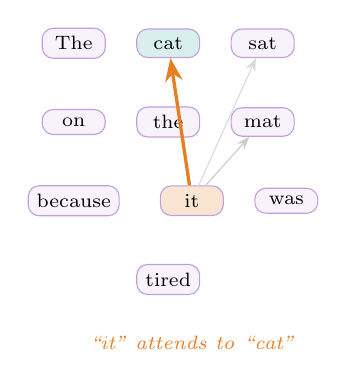
\begin{tikzpicture}[
        word/.style={draw=aiViolet!40, fill=aiViolet!5, rounded corners,
          font=\scriptsize, inner sep=3pt, minimum width=0.8cm},
        >=Stealth
      ]
        \node[word] (w1) at (0,4) {The};
        \node[word, fill=linalgTeal!15] (w2) at (1.2,4) {cat};
        \node[word] (w3) at (2.4,4) {sat};
        \node[word] (w4) at (0,3) {on};
        \node[word] (w5) at (1.2,3) {the};
        \node[word] (w6) at (2.4,3) {mat};
        \node[word] (w7) at (0,2) {because};
        \node[word, fill=accentOrange!20] (w8) at (1.5,2) {it};
        \node[word] (w9) at (2.7,2) {was};
        \node[word] (w10) at (1.2,1) {tired};

        % Attention arrows
        \draw[->,very thick,accentOrange] (w8) -- (w2);
        \draw[->,thin,gray!40] (w8) -- (w6);
        \draw[->,thin,gray!30] (w8) -- (w3);

        \node[font=\scriptsize\itshape,text=accentOrange] at (1.5,0.2)
          {``it'' attends to ``cat''};
      \end{tikzpicture}
    \end{column}
  \end{columns}

  \note{
    NOW: When your AI reads ``it'' in a sentence, self-attention lets it look at
    every other word and decide what ``it'' means.
    THEN: This equation combines Gibbs's dot product (1881), Boltzmann's softmax
    (1870s), and Cayley's matrix multiplication (1858). Three centuries of math,
    one line of code.

    ``Self-attention IS the convergence point. The dot product from Gibbs.
    The softmax from Boltzmann. The matrix multiplication from Cayley.
    All in one equation.''
  }
\end{frame}


% ============================================================
% SLIDE 23: One Transformer Layer
% ============================================================
\begin{frame}{One Transformer Layer --- The Full Stack}

  \begin{center}
    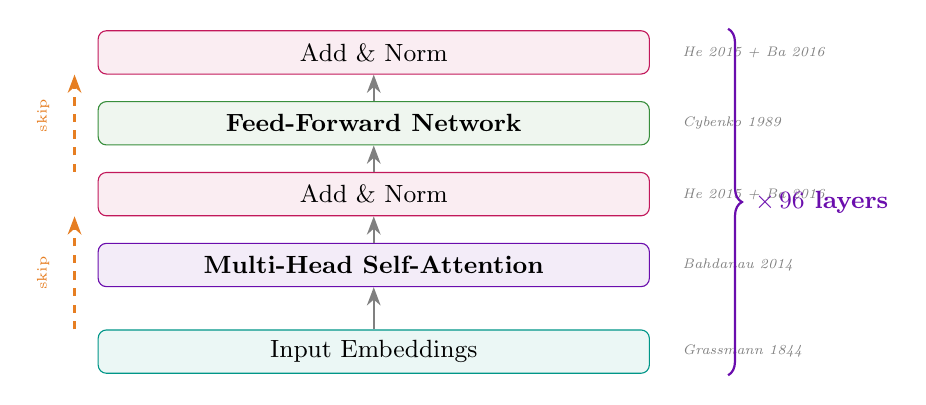
\begin{tikzpicture}[
      lbl/.style={font=\tiny\itshape, text=gray},
      blk/.style={rounded corners=3pt, minimum width=7cm,
        minimum height=0.55cm, font=\small},
      >=Stealth
    ]
      % Stack from bottom to top
      \node[blk, draw=linalgTeal, fill=linalgTeal!8] (input) at (0,0)
        {Input Embeddings};
      \node[lbl, right] at (3.8,0) {Grassmann 1844};

      \node[blk, draw=aiViolet, fill=aiViolet!8] (attn) at (0,1.1)
        {\textbf{Multi-Head Self-Attention}};
      \node[lbl, right] at (3.8,1.1) {Bahdanau 2014};

      \node[blk, draw=neuronPink, fill=neuronPink!8] (an1) at (0,2.0)
        {Add \& Norm};
      \node[lbl, right] at (3.8,2.0) {He 2015 + Ba 2016};

      \node[blk, draw=approxGreen, fill=approxGreen!8] (ffn) at (0,2.9)
        {\textbf{Feed-Forward Network}};
      \node[lbl, right] at (3.8,2.9) {Cybenko 1989};

      \node[blk, draw=neuronPink, fill=neuronPink!8] (an2) at (0,3.8)
        {Add \& Norm};
      \node[lbl, right] at (3.8,3.8) {He 2015 + Ba 2016};

      % Arrows
      \draw[->,thick,gray] (input) -- (attn);
      \draw[->,thick,gray] (attn) -- (an1);
      \draw[->,thick,gray] (an1) -- (ffn);
      \draw[->,thick,gray] (ffn) -- (an2);

      % Skip connections
      \draw[->,thick,accentOrange,dashed]
        ([xshift=-3.8cm]input.north) -- ([xshift=-3.8cm]an1.south);
      \draw[->,thick,accentOrange,dashed]
        ([xshift=-3.8cm]an1.north) -- ([xshift=-3.8cm]an2.south);
      \node[font=\tiny,accentOrange,rotate=90] at (-4.2,1.0) {skip};
      \node[font=\tiny,accentOrange,rotate=90] at (-4.2,3.0) {skip};

      % x96 bracket
      \draw[decorate, decoration={brace, amplitude=5pt, mirror},
        thick, aiViolet]
        (4.5,-0.3) -- (4.5,4.1)
        node[midway, right=6pt, font=\small\bfseries, text=aiViolet]
        {$\times\, 96$ layers};
    \end{tikzpicture}
  \end{center}

  \vspace{-0.2em}
  {\small\centering Every component was taught in an earlier slide.\par}

  \note{
    NOW: Your AI stacks 96 copies of this exact block.
    THEN: Every piece is labeled with its inventor --- Bahdanau 2014,
    He 2015, Ba 2016, Cybenko 1989. You have already met every one of them.

    ``One transformer layer: attention, then a feed-forward network, with two
    rounds of add-and-normalize. Stack 96 of these and you have GPT-4.''
  }
\end{frame}


% ============================================================
% SLIDE 24: THE CLIMAX -- Annotated Transformer -- INTERACTIVE
% ============================================================
\begin{frame}{The Full Annotated Transformer}

  \begin{columns}[T]
    \begin{column}{0.52\textwidth}
      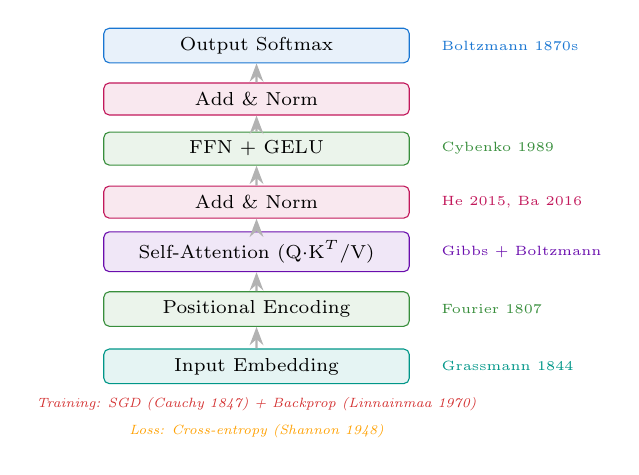
\begin{tikzpicture}[scale=0.97, every node/.style={transform shape},
        comp/.style={rounded corners=2pt, minimum width=4cm,
          minimum height=0.42cm, font=\scriptsize},
        >=Stealth
      ]
        \node[comp, draw=linalgTeal, fill=linalgTeal!10] (emb) at (0,0)
          {Input Embedding};
        \node[font=\tiny, text=linalgTeal, right] at (2.3,0)
          {Grassmann 1844};

        \node[comp, draw=approxGreen, fill=approxGreen!10] (pos) at (0,0.75)
          {Positional Encoding};
        \node[font=\tiny, text=approxGreen, right] at (2.3,0.75)
          {Fourier 1807};

        \node[comp, draw=aiViolet, fill=aiViolet!10] (sa) at (0,1.5)
          {Self-Attention (Q$\cdot$K$^T$/V)};
        \node[font=\tiny, text=aiViolet, right] at (2.3,1.5)
          {Gibbs + Boltzmann};

        \node[comp, draw=neuronPink, fill=neuronPink!10] (an1) at (0,2.15)
          {Add \& Norm};
        \node[font=\tiny, text=neuronPink, right] at (2.3,2.15)
          {He 2015, Ba 2016};

        \node[comp, draw=approxGreen, fill=approxGreen!10] (ffn) at (0,2.85)
          {FFN + GELU};
        \node[font=\tiny, text=approxGreen, right] at (2.3,2.85)
          {Cybenko 1989};

        \node[comp, draw=neuronPink, fill=neuronPink!10] (an2) at (0,3.5)
          {Add \& Norm};

        \node[comp, draw=probBlue, fill=probBlue!10] (soft) at (0,4.2)
          {Output Softmax};
        \node[font=\tiny, text=probBlue, right] at (2.3,4.2)
          {Boltzmann 1870s};

        % Arrows
        \draw[->,thick,gray!60] (emb) -- (pos);
        \draw[->,thick,gray!60] (pos) -- (sa);
        \draw[->,thick,gray!60] (sa) -- (an1);
        \draw[->,thick,gray!60] (an1) -- (ffn);
        \draw[->,thick,gray!60] (ffn) -- (an2);
        \draw[->,thick,gray!60] (an2) -- (soft);

        % Training annotations below
        \node[font=\tiny\itshape, text=calculusRed] at (0,-0.5)
          {Training: SGD (Cauchy 1847) + Backprop (Linnainmaa 1970)};
        \node[font=\tiny\itshape, text=infoAmber] at (0,-0.85)
          {Loss: Cross-entropy (Shannon 1948)};
      \end{tikzpicture}
    \end{column}

    \begin{column}{0.45\textwidth}
      % Interactive moment
      \begin{tcolorbox}[colback=accentOrange!10, colframe=accentOrange,
        fonttitle=\bfseries, title={\faUsers\ Interactive Moment},
        rounded corners, boxrule=1pt, left=3pt, right=3pt, top=2pt, bottom=2pt]
        \centering\small
        Count the building blocks.\\[6pt]
        How many of the 10 sections\\
        can you find in this diagram?\\[6pt]
        {\scriptsize Each component was invented by\\
         someone you just met.}
      \end{tcolorbox}

      \vspace{0.2em}
      \begin{tcolorbox}[colback=aiViolet!8, colframe=aiViolet,
        boxrule=1pt, rounded corners, left=4pt, right=4pt, top=4pt, bottom=4pt]
        \centering\small
        \textbf{2,000 years of mathematics,}\\
        \textbf{all running at once.}\\[4pt]
        \scriptsize
        1807 \textperiodcentered{} 1844 \textperiodcentered{} 1847
        \textperiodcentered{} 1858 \textperiodcentered{} 1870s
        \textperiodcentered{} 1881\\
        1943 \textperiodcentered{} 1948 \textperiodcentered{} 1970
        \textperiodcentered{} 1986 \textperiodcentered{} 1989\\
        2013 \textperiodcentered{} 2014 \textperiodcentered{} 2015
        \textperiodcentered{} 2016 \textperiodcentered{} 2017
      \end{tcolorbox}
    \end{column}
  \end{columns}

  \note{
    NOW: This is the complete machine. Every word your AI says passes through
    this pipeline. THEN: [Gesture at annotations.] 1807. 1844. 1847. 1858.
    1870s. 1948. 1970. 1989. 2013. 2014. 2015. 2016. 2017.
    Two thousand years of human invention, all running at once.

    INTERACTIVE MOMENT 3 ($\sim$3 minutes): ``Count the building blocks.
    Look at this diagram and identify which of the 10 sections each component
    comes from. How many can you find?''

    [PAUSE. Let the diagram land.]
  }
\end{frame}


% ============================================================
% SLIDE 25: Positional Encoding + Convergence
% ============================================================
\begin{frame}{Positional Encoding --- Fourier Inside the Transformer}

  \begin{columns}[T]
    \begin{column}{0.52\textwidth}
      % Positional encoding explanation
      \begin{tcolorbox}[colback=approxGreen!5, colframe=approxGreen,
        fonttitle=\bfseries\small,
        title={Same Math, 210 Years Apart},
        rounded corners, boxrule=0.8pt, left=3pt, right=3pt, top=2pt, bottom=2pt]
        \small
        \textbf{Fourier} (1807): Decompose heat into waves.\\[4pt]
        \textbf{Vaswani} (2017): Decompose word position into waves.\\[6pt]
        $PE_{(pos,2i)} = \sin\!\left(\dfrac{pos}{10000^{2i/d}}\right)$\\[6pt]
        $PE_{(pos,2i+1)} = \cos\!\left(\dfrac{pos}{10000^{2i/d}}\right)$
      \end{tcolorbox}

      \vspace{0.2em}
      % Positional encoding waves
      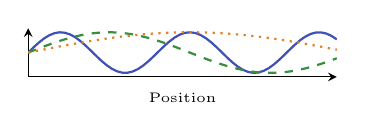
\begin{tikzpicture}
        \begin{axis}[
          width=5.5cm, height=2.2cm,
          domain=0:30, samples=60,
          axis lines=left,
          xlabel={\tiny Position},
          ylabel={},
          ymin=-1.2, ymax=1.2,
          xtick=\empty, ytick=\empty,
          every axis plot/.append style={thick, no markers}
        ]
          \addplot[seqIndigo] {sin(deg(x/2))};
          \addplot[approxGreen, dashed] {sin(deg(x/5))};
          \addplot[accentOrange, dotted] {sin(deg(x/10))};
        \end{axis}
      \end{tikzpicture}

      {\scriptsize\centering Different frequencies $=$ different position scales.\par}
    \end{column}

    \begin{column}{0.45\textwidth}
      \convergencebar{9}

      \vspace{0.15em}
      {\small\bfseries Nine nodes lit. One to go.}

      \vspace{0.3em}
      \begin{insightbox}
        \small
        Your AI knows that ``dog bites man'' and ``man bites dog'' are different
        because of positional encoding.

        \vspace{0.2em}
        Fourier's sine waves, repurposed.
      \end{insightbox}

      \vspace{0.15em}
      {\small\itshape The architecture is ready.\\Now: scale it up.}
    \end{column}
  \end{columns}

  \note{
    NOW: Your AI knows word order because of positional encoding.
    THEN: 1807, Paris --- Fourier decomposes heat into sine waves.
    2017, Google --- Vaswani decomposes word position into the same sine waves.
    Same math, 210 years apart.

    ``One detail we skipped: the transformer has no built-in notion of word
    order. Vaswani added sine and cosine functions at different frequencies.
    Fourier's idea, applied directly.''
  }
\end{frame}


% ============================================================
% SLIDE 26: Scaling Laws
% ============================================================
\section{Scaling}
\begin{frame}{Scaling Laws --- Same Architecture, Just Bigger}

  \begin{columns}[T]
    \begin{column}{0.48\textwidth}
      % GPT timeline table
      \begin{tcolorbox}[colback=accentOrange!5, colframe=accentOrange,
        fonttitle=\bfseries\small, title={The Scaling Explosion},
        rounded corners, boxrule=0.8pt, left=3pt, right=3pt, top=2pt, bottom=2pt]
        \scriptsize
        \begin{tabular}{@{}lcr@{}}
          \toprule
          \textbf{Model} & \textbf{Year} & \textbf{Parameters} \\
          \midrule
          GPT-1 & 2018 & 117M \\
          GPT-2 & 2019 & 1.5B \\
          GPT-3 & 2020 & 175B \\
          GPT-4 & 2023 & undisclosed \\
          Claude 3.5 & 2024 & undisclosed \\
          \bottomrule
        \end{tabular}\\[6pt]
        Same 2017 blueprint. 1,500$\times$ larger.
      \end{tcolorbox}

      \vspace{0.2em}
      {\scriptsize Kaplan et al.\ (2020): performance scales as a smooth power law
       with parameters, data, and compute.}
    \end{column}

    \begin{column}{0.49\textwidth}
      % Semilog scaling chart
      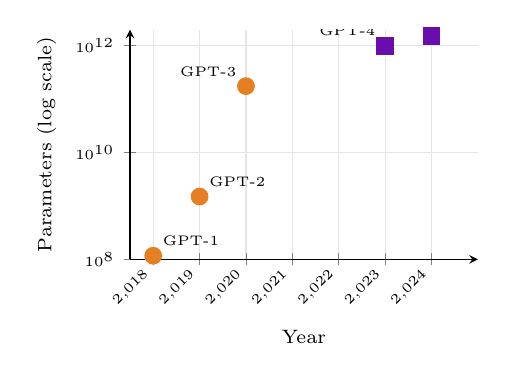
\begin{tikzpicture}
        \begin{axis}[
          width=6cm, height=4.5cm,
          xlabel={\scriptsize Year},
          ylabel={\scriptsize Parameters (log scale)},
          ymode=log,
          xmin=2017.5, xmax=2025,
          ymin=1e8, ymax=2e12,
          xtick={2018,2019,2020,2021,2022,2023,2024},
          x tick label style={font=\tiny, rotate=45, anchor=east},
          y tick label style={font=\tiny},
          grid=major,
          grid style={gray!20},
          axis lines=left,
        ]
          \addplot[only marks, mark=*, mark size=3pt, accentOrange]
            coordinates {
              (2018, 1.17e8)
              (2019, 1.5e9)
              (2020, 1.75e11)
            };
          \addplot[only marks, mark=square*, mark size=3pt, aiViolet]
            coordinates {
              (2023, 1e12)
              (2024, 1.5e12)
            };
          % Labels
          \node[font=\tiny, above right] at (axis cs:2018, 1.17e8) {GPT-1};
          \node[font=\tiny, above right] at (axis cs:2019, 1.5e9) {GPT-2};
          \node[font=\tiny, above left] at (axis cs:2020, 1.75e11) {GPT-3};
          \node[font=\tiny, above left] at (axis cs:2023, 1e12) {GPT-4};
        \end{axis}
      \end{tikzpicture}
    \end{column}
  \end{columns}

  \note{
    NOW: GPT-4, Claude, Gemini --- all the same 2017 architecture, just scaled up.
    THEN: 2018 --- GPT-1, 117 million parameters. 2020 --- GPT-3, 175 billion.
    Same blueprint, 1,500$\times$ larger. The math didn't change. The scale did.

    ``Somewhere along the way, these models started doing things nobody programmed
    them to do --- reasoning, writing code, translating languages they were barely
    trained on.''
  }
\end{frame}


% ============================================================
% SLIDE 27: The Current Landscape
% ============================================================
\begin{frame}{Return to the Diagram --- Now You Understand}

  \begin{center}
    \begin{tcolorbox}[colback=aiViolet!5, colframe=aiViolet,
      fonttitle=\bfseries\small, title={The Complete Inventory},
      rounded corners, boxrule=1pt, width=0.92\textwidth,
      left=4pt, right=4pt, top=3pt, bottom=3pt]
      \scriptsize
      \begin{tabular}{@{}lll@{}}
        \toprule
        \textbf{Component} & \textbf{Inventor(s)} & \textbf{Date} \\
        \midrule
        Embedding & Grassmann, Mikolov & 1844, 2013 \\
        Positional encoding & Fourier, Vaswani & 1807, 2017 \\
        Self-attention (dot product) & Gibbs, Bahdanau & 1881, 2014 \\
        Softmax & Boltzmann & 1870s \\
        Matrix multiplication & Cayley & 1858 \\
        Add \& Norm & He, Ba & 2015, 2016 \\
        Feed-forward + GELU & Cybenko, Hendrycks & 1989, 2016 \\
        Output softmax & Boltzmann/Luce & 1870s \\
        Gradient descent & Cauchy & 1847 \\
        Backpropagation & Linnainmaa, Hinton & 1970, 1986 \\
        Cross-entropy loss & Shannon & 1948 \\
        \bottomrule
      \end{tabular}
    \end{tcolorbox}

    \vspace{0.3em}
    {\small At the start, this was overwhelming. Now you can point to each piece\\
     and say \textbf{who} invented it, \textbf{when}, and \textbf{why}.}
  \end{center}

  \note{
    NOW: You can read this diagram. Every piece has a name, a date, a person.
    THEN: Look at the dates --- 1807, 1844, 1847, 1858, 1870s, 1881, 1943,
    1948, 1970, 1986, 1989, 2013, 2014, 2015, 2016, 2017.
    Centuries of work, all running in the machine in your pocket.

    ``At the start of this lecture, this diagram was overwhelming. Now you
    can point to each piece and say who invented it, when, and why.''
  }
\end{frame}


% ============================================================
% SLIDE 28: Full Convergence Diagram
% ============================================================
\begin{frame}{Full Convergence --- All Ten Streams}

  \convergencebar{10}

  \begin{center}
  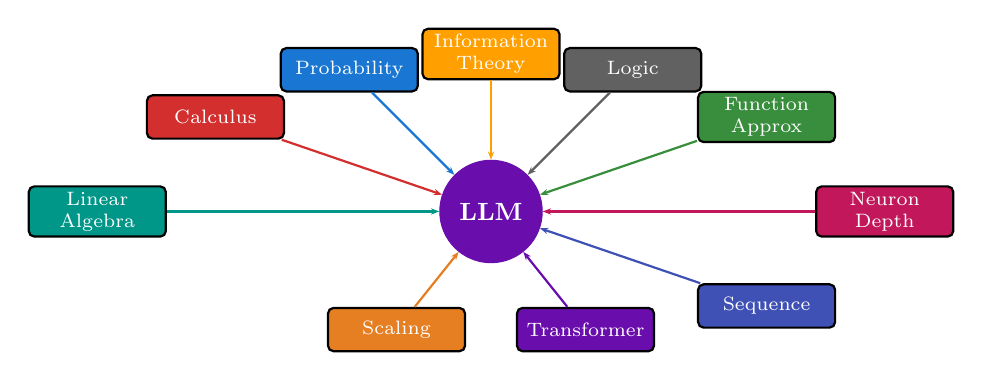
\begin{tikzpicture}[
    every node/.style={font=\scriptsize, align=center, minimum height=0.55cm,
      rounded corners=2pt, inner sep=2pt},
    lit/.style={draw, thick, text=white}
  ]
    \node[lit, fill=linalgTeal, text width=1.6cm] (n1) at (-5,0) {Linear\\Algebra};
    \node[lit, fill=calculusRed, text width=1.6cm] (n2) at (-3.5,1.2) {Calculus};
    \node[lit, fill=probBlue, text width=1.6cm] (n3) at (-1.8,1.8) {Probability};
    \node[lit, fill=infoAmber, text width=1.6cm] (n4) at (0,2) {Information\\Theory};
    \node[lit, fill=logicGray, text width=1.6cm] (n5) at (1.8,1.8) {Logic};
    \node[lit, fill=approxGreen, text width=1.6cm] (n6) at (3.5,1.2) {Function\\Approx};
    \node[lit, fill=neuronPink, text width=1.6cm] (n7) at (5,0) {Neuron\\Depth};
    \node[lit, fill=seqIndigo, text width=1.6cm] (n8) at (3.5,-1.2) {Sequence};
    \node[lit, fill=aiViolet, text width=1.6cm] (n9) at (1.2,-1.5) {Transformer};
    \node[lit, fill=accentOrange, text width=1.6cm] (n10) at (-1.2,-1.5) {Scaling};
    % Center -- now reveals TRANSFORMER
    \node[draw=aiViolet, fill=aiViolet, circle, minimum size=1.3cm,
      font=\small\bfseries, text=white] (ctr) at (0,0) {LLM};
    % Arrows from all nodes
    \draw[-{Stealth[length=3pt]}, linalgTeal, thick] (n1) -- (ctr);
    \draw[-{Stealth[length=3pt]}, calculusRed, thick] (n2) -- (ctr);
    \draw[-{Stealth[length=3pt]}, probBlue, thick] (n3) -- (ctr);
    \draw[-{Stealth[length=3pt]}, infoAmber, thick] (n4) -- (ctr);
    \draw[-{Stealth[length=3pt]}, logicGray, thick] (n5) -- (ctr);
    \draw[-{Stealth[length=3pt]}, approxGreen, thick] (n6) -- (ctr);
    \draw[-{Stealth[length=3pt]}, neuronPink, thick] (n7) -- (ctr);
    \draw[-{Stealth[length=3pt]}, seqIndigo, thick] (n8) -- (ctr);
    \draw[-{Stealth[length=3pt]}, aiViolet, thick] (n9) -- (ctr);
    \draw[-{Stealth[length=3pt]}, accentOrange, thick] (n10) -- (ctr);
  \end{tikzpicture}
  \end{center}

  \vspace{-0.3em}
  {\large\centering\bfseries Ten streams of human invention, flowing into one machine.\par}

  \note{
    NOW: This is the complete picture --- every branch of mathematics that runs
    inside your AI. THEN: 2,000+ years of human curiosity, from Archimedes
    to Vaswani, converging in one architecture.

    [Let the diagram speak. Pause.]
    ``Ten streams of human invention, flowing into one machine.''
  }
\end{frame}


% ============================================================
% SLIDE 29: Open Questions
% ============================================================
\section{Closing}
\begin{frame}{The Story Is Not Over}

  \begin{columns}[T]
    \begin{column}{0.48\textwidth}
      \begin{tcolorbox}[colback=aiViolet!5, colframe=aiViolet,
        fonttitle=\bfseries\small, title={Open Questions},
        rounded corners, boxrule=1pt, left=4pt, right=4pt, top=4pt, bottom=4pt]
        \small
        \textbf{Why} do transformers work so well?\\
        No one fully knows.\\[6pt]
        \textbf{What are the limits} of scaling?\\
        Are we near the ceiling or far from it?\\[6pt]
        \textbf{What comes after} transformers?\\
        State space models? Hybrid architectures?\\[6pt]
        \textbf{What new math} will be needed?\\
        The tools may not exist yet.
      \end{tcolorbox}
    \end{column}

    \begin{column}{0.49\textwidth}
      \vspace{1em}
      \begin{tcolorbox}[colback=accentOrange!8, colframe=accentOrange,
        fonttitle=\bfseries, title={Perspective},
        rounded corners, boxrule=1pt, left=4pt, right=4pt, top=4pt, bottom=4pt]
        \small
        The math is 2,000 years old.

        \vspace{0.3em}
        The architecture is only \textbf{8 years old}.

        \vspace{0.3em}
        There are open questions everywhere.

        \vspace{0.5em}
        Every breakthrough we covered today started with someone
        asking a question nobody else was asking.

        \vspace{0.3em}
        The next breakthrough will start the same way.
      \end{tcolorbox}
    \end{column}
  \end{columns}

  \note{
    NOW: Transformers power everything, but nobody fully understands why
    they work this well. THEN: Every breakthrough we covered today started
    with someone asking a question nobody else was asking.
    The next breakthrough will start the same way.

    ``The transformer is not the end of the story. It's the latest chapter.
    The people who will answer these questions might be sitting in this room.''
  }
\end{frame}


% ============================================================
% SLIDE 30: Closing -- Your Turn
% ============================================================
\begin{frame}[plain]
  \begin{tikzpicture}[remember picture, overlay]
    \fill[aiViolet] (current page.south west) rectangle (current page.north east);
  \end{tikzpicture}

  \vspace{0.3cm}
  \begin{columns}[T]
    \begin{column}{0.45\textwidth}
      \begin{center}
        \textcolor{white!80}{\large\itshape 1943}\\[6pt]
        \textcolor{white!90}{\small McCulloch \& Pitts draw\\
          a single neuron on paper.}
      \end{center}
    \end{column}
    \begin{column}{0.1\textwidth}
      \begin{center}
        \vspace{0.5em}
        \textcolor{white!50}{\rule{0.5pt}{3cm}}
      \end{center}
    \end{column}
    \begin{column}{0.45\textwidth}
      \begin{center}
        \textcolor{white!80}{\large\itshape 2026}\\[6pt]
        \textcolor{white!90}{\small Trillion-parameter models\\
          reason, write, and create.}
      \end{center}
    \end{column}
  \end{columns}

  \vspace{1em}
  \begin{center}
    {\Huge\bfseries\textcolor{white}{The math your generation will create}}\\[0.4em]
    {\Huge\bfseries\textcolor{accentOrange}{is not written yet.}}
  \end{center}

  \vspace{1em}
  {\small\centering\textcolor{white!60}{2,000+ Years of Mathematics.
   One Machine. \textbf{Your Turn.}}\par}

  \vspace{0.3em}
  {\footnotesize\centering\textcolor{white!40}{Prof.\ J.\ Osterrieder
   \hspace{2em} 2026}\par}

  \note{
    NOW: You understand the machine. Every piece, every inventor, every date.
    THEN: They all started by following their curiosity. Your turn.

    ``Every piece of mathematics we covered today was invented by someone who
    had no idea it would end up inside an AI. Grassmann was a schoolteacher.
    Pascal was answering a gambling question. Fourier was studying heat.
    Boltzmann was studying gas molecules. They followed their curiosity and
    built the future. The next great idea might come from you. Thank you.''
  }
\end{frame}


\end{document}
